\documentclass[twocolumn]{article}

% --- Core Layout & Spacing ---
\usepackage[final]{graphicx} 
\usepackage[utf8]{inputenc} 
\usepackage[T1]{fontenc}    
\usepackage{geometry}       
\geometry{letterpaper, top=0.75in, bottom=0.75in, left=0.75in, right=0.75in, columnsep=0.25in}

% --- 1. LOAD AUTHBLK FIRST ---
\usepackage{authblk} 
\usepackage{cuted} % For spanning abstract across two columns

% --- 2. DEFINE THE AUTHORS USING EXPLICIT BRACKETS ---
\author[1]{\textbf{Anis Ur Rahman}}
\author[2]{\textbf{Mete Ahishali}}
\author[3]{\textbf{Einari Heinaro}}
\author[2,4]{\textbf{Samuli Junttila}}
\affil[1]{CSC -- IT Center for Science Ltd., Espoo, Finland}
\affil[2]{Department of Forest Sciences, University of Helsinki}
\affil[3]{KOKO Forest Ltd.}
\affil[4]{School of Forest Sciences, University of Eastern Finland}
\affil[ ]{\texttt{anis.rahman@csc.fi, mete.ahishali@helsinki.fi, einari.heinaro@kokoforest.com, samuli.junttila@\{helsinki,uef\}.fi}}

% --- Other Essential CS Packages ---
\usepackage{amsmath, amssymb, amsthm} 
\usepackage{booktabs}                 
\usepackage{microtype}                
\usepackage{url}                      
\usepackage{hyperref}                 
\hypersetup{colorlinks=true, linkcolor=blue, urlcolor=cyan, citecolor=green}

% --- Document Formatting Customizations ---
\usepackage{natbib} % Flexible bibliography management
\setcitestyle{numbers,square}

% --- Metadata ---
\title{\textbf{Cross-Domain Dead Tree Detection via Knowledge Distillation in Aerial Imagery}}

\date{} % Leave empty to omit date

\newcommand{\red}[1]{{\color{red}#1}}
\newcommand{\todo}[1]{{\color{red}#1}}
\newcommand{\TODO}[1]{\textbf{\color{red}[TODO: #1]}}
\newcommand{\mypar}[1]{\noindent\textbf{#1}}

\usepackage{makecell}
\renewcommand\theadfont{\bfseries\scshape}% applied to every line of \thead
\newcommand{\myhdr}[2][c]{\thead[#1]{#2}}

\usepackage{duckuments}
\usepackage{comment}
\usepackage{xspace}

\newcommand{\anis}[1]{{\color{magenta} {[AR] #1}}}
\newcommand{\einari}[1]{{\color{teal} {[EH] #1}}}
\newcommand{\mete}[1]{{\color{orange} {[MA] #1}}}
\newcommand{\samuli}[1]{{\color{blue} {[SJ] #1}}}

\usepackage{lineno}

\usepackage{amsmath}
\usepackage{amsfonts}

\usepackage{booktabs}
\usepackage{tabularx}
\usepackage{adjustbox}
\usepackage{multicol}
\usepackage{multirow}
\usepackage{caption}
\newcommand{\rotate}[3]{\rotatebox[origin=#1]{#2}{#3}}

\usepackage{subcaption}

\newcommand{\params}{\theta}
\newcommand{\classifier}{\phi}
\newcommand{\Classifier}{\Phi}

\newcommand{\paramsT}{\params_t}
\newcommand{\paramsV}{\params_v}
\newcommand{\paramsSp}{\omega}
\newcommand{\paramsSpT}{\paramsSp_t}
\newcommand{\paramsSpV}{\paramsSp_v}

\newcommand{\paramsSpLN}{\omega_\mathtt{LN}}
\newcommand{\paramsSpLNOptim}{\omega_\mathtt{LN}^*}
\newcommand{\paramsSpLNT}{\paramsSpLN^t}
\newcommand{\paramsSpLNV}{\paramsSpLN^v}
\newcommand{\paramsSpLNTOptim}{\paramsSpLN^{*^t}}
\newcommand{\paramsSpLNVOptim}{\paramsSpLN^{*^v}}

\newcommand{\vlm}{f}
\newcommand{\vlmP}{\vlm_\params}
\newcommand{\vlmV}{\vlm^v}
\newcommand{\vlmT}{\vlm^t}
\newcommand{\vlmVP}{\vlmV_{\params_v}}
\newcommand{\vlmTP}{\vlmT_{\params_t}}

\newcommand{\vlmVSP}{\vlmV_{\paramsSpV}}
\newcommand{\vlmTSP}{\vlmT_{\paramsSpT}}

\newcommand{\vlmVSPOptim}{\vlmV_{\paramsSpV^*}}
\newcommand{\vlmTSPOptim}{\vlmT_{\paramsSpT^*}}

\newcommand{\vlmVLN}{\vlmV_{\paramsSpLNV}}
\newcommand{\vlmTLN}{\vlmT_{\paramsSpLNT}}

\newcommand{\vlmVLNOptim}{\vlmV_{\paramsSpLNVOptim}}
\newcommand{\vlmTLNOptim}{\vlmT_{\paramsSpLNTOptim}}

\newcommand{\textSpace}{\mathcal{T}}
\newcommand{\imageSpace}{\mathcal{I}}
\newcommand{\embedSpace}{\mathbb{R}^d}

\newcommand{\cossim}{\text{sim}}

\newcommand{\imageIn}{x}
\newcommand{\labelIn}{y}
\newcommand{\genClass}{c}
\newcommand{\baseClass}{b}
\newcommand{\genString}{s_c}
\newcommand{\baseClasses}{\mathcal{B}}
\newcommand{\novelClasses}{\mathcal{N}}
\newcommand{\genClasses}{\mathcal{C}}

\newcommand{\dataset}{D}
\newcommand{\datasetSize}{n}
\newcommand{\niter}{m}
\newcommand{\shots}{k}
\newcommand{\pairDataId}[1]{(\imageIn_#1,\labelIn_#1)}
\newcommand{\pairData}{(\imageIn,\labelIn)}

\DeclareMathOperator*{\argmax}{arg\,max}
\DeclareMathOperator*{\argmin}{arg\,min}

\newcommand{\oursone}{\textit{TreeMort-1T-UNet}\xspace}
\newcommand{\oursthree}{\textit{TreeMort-3T-UNet}\xspace}

\newcommand{\ourslora}{\ours{}\textsubscript{\texttt{LoRA}}}
\newcommand{\oursln}{\ours{}\textsubscript{\texttt{LayerNorm}}}

\usepackage{pifont}

\usepackage[table]{xcolor}
\definecolor{lncolor}{HTML}{FEE4C4}
\definecolor{baseline}{HTML}{E0E4E8}
\definecolor{ppink}{rgb}{0.98, 0.575, 0.89}


\begin{document}

% Strip abstract across two columns
\twocolumn[
  \begin{center}
    \maketitle
    \begin{abstract}
    Detecting dead trees in aerial imagery is vital for assessing forest health, yet domain variability and scarce labeled data severely limit model generalization across diverse forest ecosystems. We present a systematic benchmark of four knowledge distillation (KD) strategies --- Basic, Self, Feature-level, and Ensemble --- for cross-domain dead tree detection using the \oursone (Tree Mortality 1-Task U-Net) model, evaluated across three target domains (Poland, Germany, Estonia) with a Finnish teacher achieving Tree IoU of 0.448 on the source domain. All four KD variants substantially outperform direct fine-tuning: Self KD leads on Poland (Tree IoU 0.277 vs.\ 0.216) and Germany (0.328 vs.\ 0.108), while Feature-level KD achieves the highest cross-domain stability on Estonia (0.265 vs.\ 0.202). We compare against domain-adversarial neural network (DANN) training with gradient-reversal feature alignment~\citep{ganin2016domain}; all KD variants outperform DANN on every target country (e.g., Poland: KD 0.277 vs.\ DANN 0.242), demonstrating that teacher-guided soft-target transfer is more effective than adversarial domain alignment when labeled target data is available. Feature-level KD's intermediate feature alignment yields the most consistent centroid precision across domains and superior representational invariance (higher deep-layer CKA, better domain mixing in t-SNE, linear probing AUC 0.95), making it the preferred strategy for precision-critical forestry applications. These results establish Self KD and Feature-level KD as reliable, scalable transfer strategies for ecological dead tree mapping across European boreal and temperate forests.
    \end{abstract}
    \vspace{0.3in}
  \end{center}
]

% %%Graphical abstract
% \begin{graphicalabstract}
% %\includegraphics{grabs}
% \end{graphicalabstract}

% %%Research highlights
% \begin{highlights}
% \item Pioneering KD enhances dead tree detection across forest domains.
% \item \textit{Feature-level KD} delivers robust precision for ecological monitoring.
% \item Novel analyses prove KD's scalability in climate-challenged forests.
% \end{highlights}

% %% Keywords
% \begin{keyword}
% Dead tree segmentation \sep forest mortality mapping \sep aerial imagery analysis \sep knowledge distillation \sep domain adaption
% \end{keyword}

\section{Introduction}
\label{sec:intro}

Dead trees are critical indicators of forest health, biodiversity, and wildfire risk, with global tree mortality increasing due to climate change-driven factors such as intensified droughts, heat extremes, insect outbreaks, and wildfires, leading to widespread forest die-off and urgent needs for enhanced monitoring~\citep{junttila2024significant,cheng2024scattered,international2025towards}. Their detection through remote sensing is therefore essential for environmental monitoring and effective forestry management, as field surveys are often infeasible due to limited accessibility, high costs, and the scattered occurrence of dead trees across vast areas, while remote sensing offers efficiency, scalability, and comprehensive coverage for mapping individual dead trees. High-resolution aerial imagery enables the precise identification of individual dead trees across large forest areas, revealing mortality patterns increasingly linked to climate change~\citep{ahishali2025ada}. However, this task presents significant challenges. Dense canopy cover and spectral similarities between living and dead vegetation often hinder accurate segmentation~\citep{briechle2021silvi}. Moreover, \textbf{domain variability} poses a substantial obstacle, as models trained on one forest region frequently fail to generalize to others due to differences in tree species, terrain, and imaging conditions~\citep{angarano2024domain}. For instance, dead conifers in Finland's sparse boreal forests are easily distinguishable against open canopies, whereas decaying broadleaves in Poland's dense temperate forests are often obscured by surrounding foliage and variable lighting. These challenges are compounded by \textbf{data scarcity}, as annotated datasets are limited by the high cost of expert labeling and the infrequent occurrence of dead trees in certain regions~\citep{kellenberger2018detecting, liu2019knowledge}.

Traditional transfer learning methods, such as fine-tuning pre-trained models, often prove inadequate in this context. Fine-tuning requires labeled data from the target domain, which is frequently unavailable, and it struggles with significant distribution shifts, leading to overfitting or the loss of generalizable features~\citep{tuia2016domain}. Recent domain adaptation techniques in remote sensing, such as image-to-image translation, aim to align data across different sites~\citep{wang2019domain, ahishali2025ada}. Although these methods have shown promise for tasks like cross-site tree mortality mapping~\citep{chen2022object, dalponte2019individual}, they often involve complex training processes and fail to fully leverage the knowledge embedded in segmentation models.

To overcome these limitations, we propose \textbf{knowledge distillation (KD)} as an effective strategy for improving cross-domain generalization in dead tree segmentation. KD enables a compact student model to learn from a robust teacher model, absorbing both class labels and subtle insights from the teacher's outputs~\citep{hinton2015distilling}. Through this process, the student model learns to capture domain-invariant features, such as textural signs of decay, while adapting to region-specific differences. Unlike fine-tuning, KD uses a teacher model trained on a well-annotated source domain (e.g., Finnish aerial imagery) to guide the student's learning on an unseen target domain (e.g., Polish imagery), reducing the need for extensive retraining. This approach not only addresses domain variability but also mitigates the challenges posed by scarce labeled data, making KD a scalable solution for ecological monitoring.

In this study, we benchmark KD strategies using a Finnish source domain and three target domains (Poland, Germany, Estonia), spanning boreal-to-temperate forest gradients. We also evaluate DANN as a domain adaptation baseline. Our findings demonstrate KD's capacity to bridge domain gaps and reduce dependence on site-specific annotations, consistently outperforming adversarial alignment. Specifically, our contributions are as follows:

\begin{enumerate}
\item \textbf{Multi-country benchmark:} We present the first systematic benchmark of KD strategies for cross-domain dead tree detection, evaluated across four European forest domains (Finland, Poland, Germany, Estonia) spanning boreal-to-temperate gradients with distinct imaging conditions, tree species, and annotation densities.
\item \textbf{Domain adaptation comparison:} We implement and evaluate DANN~\citep{ganin2016domain} adversarial domain alignment as a direct comparison baseline, demonstrating that all KD variants consistently outperform adversarial feature alignment across every target country.
\item \textbf{Comparative KD evaluation:} Using an updated teacher model (Tree IoU 0.448 on Finland), we reveal that teacher quality critically affects student transfer and identify Self KD and Feature-level KD as complementary strategies with distinct strengths in detection accuracy and cross-domain precision.
\item \textbf{Practical guidance:} We provide actionable guidance for forestry practitioners: Self KD maximizes detection accuracy; Feature-level KD minimizes false positives for precision-critical monitoring applications.
\end{enumerate}

The paper is structured as follows: Section~\ref{sec:related} reviews related work, Section~\ref{sec:method} outlines our methodology, Section~\ref{sec:results} presents experimental findings, Section~\ref{sec:discussion} discusses broader implications, and Section~\ref{sec:conclusion} provides concluding remarks.

\section{Related Work}
\label{sec:related}

Transfer learning and knowledge distillation have emerged as pivotal techniques in addressing the challenges of data scarcity and computational constraints in remote sensing, particularly within the domain of ecological monitoring. This section provides a comprehensive overview of the existing literature, highlighting the evolution of these methods and their application to tasks analogous to dead tree detection in aerial imagery.

\subsection{Transfer Learning in Remote Sensing}

Transfer learning, which leverages pre-trained models to adapt to new tasks or domains, has become a cornerstone in remote sensing due to the limited availability of labeled datasets. Models pre-trained on large, general-purpose datasets such as \textit{ImageNet}~\citep{deng2009imagenet} are frequently fine-tuned for specific remote sensing tasks, including land cover classification~\citep{xie2016transfer}, object detection~\citep{chen2022object}, and semantic segmentation~\citep{zhang2016deep}. For instance, Xie et al.~\citep{xie2016transfer} demonstrated that fine-tuning a \textit{CNN} pre-trained on \textit{ImageNet} significantly improves classification accuracy on satellite imagery, even with small training sets. However, the efficacy of such approaches diminishes when confronted with pronounced domain shifts, as is common in forestry applications where spectral and structural variability across regions can be substantial~\citep{tuia2016domain}.

In the context of forestry, transfer learning has been applied to tasks such as tree species classification~\citep{kellenberger2018detecting} and estimation of forest structural variables~\citep{fassnacht2016review}. \cite{kellenberger2018detecting} utilized a fine-tuned \textit{ResNet} model to classify tree species in UAV imagery, achieving notable accuracy improvements over training from scratch. Nonetheless, these studies often assume a degree of domain similarity that may not hold for dead tree detection, where the visual signatures of decay are subtle and highly variable across ecosystems.

\subsection{Knowledge Distillation: Principles and Applications}

Knowledge distillation~\citep{hinton2015distilling} extends the paradigm of transfer learning by enabling the transfer of learned representations from a larger, pre-trained ``teacher" model to a smaller, more efficient ``student" model. This technique not only facilitates model compression but also enhances generalization by leveraging the teacher's so-called \textit{dark knowledge}, i.e., the implicit relationships encoded in its output probabilities. Distillation has been widely adopted in computer vision for tasks such as image classification~\citep{romero2014fitnets} and object detection~\citep{chen2017learning}, where it has been shown to improve both accuracy and inference speed.

In remote sensing, knowledge distillation has been explored for applications including land cover mapping~\citep{liu2019knowledge} and hyperspectral image analysis~\citep{wang2019domain}. For example, \cite{liu2019knowledge} employed distillation to compress a large \textit{CNN} for land cover classification, achieving comparable accuracy with a fraction of the computational cost. However, the application of distillation to more specialized tasks, such as dead tree detection, remains underexplored. The unique challenges of this task, such as the need to discern fine-grained, domain-specific features, necessitate tailored distillation strategies that go beyond standard output-level supervision.

\subsection{Dead Tree Detection: Challenges and Existing Approaches}

The detection of dead trees in aerial imagery is a particularly demanding task due to several factors:

\begin{itemize}
\item \textbf{Spectral Similarity:} Dead trees often exhibit spectral signatures that closely resemble those of living trees or other vegetation in early decay stages~\citep{meddens2011evaluating}, but in later stages, they may be more similar to bare ground or rocks due to foliage loss, particularly in infrared regions, leading to classification challenges~\citep{zielewska2020detection,liu2021mapping}.
\item \textbf{Occlusion and Clutter:} Dense forest canopies can obscure dead trees, while cluttered backgrounds complicate segmentation~\citep{dalponte2019individual}.
\item \textbf{Domain Variability:} Variations in tree species, terrain, imaging conditions, and decay stages across different regions exacerbate the generalization problem~\citep{fassnacht2014comparison}. For instance, dead trees in early decay resemble living vegetation, while long-standing dead trees with few remaining branches are notably harder to detect due to their sparse appearance.
\end{itemize}

Existing methods for dead tree detection range from traditional image processing techniques, such as thresholding and edge detection~\citep{garrity2013quantifying}, to more advanced machine learning approaches~\citep{polewski2018learning}. However, these methods frequently rely on handcrafted features or require extensive domain-specific tuning, limiting their applicability across diverse forest ecosystems. Recent studies have begun to explore deep learning for this task~\citep{briechle2021silvi}, yet they often overlook the critical issue of domain adaptation, assuming access to large, region-specific labeled datasets.

\subsection{Positioning of the Current Work}

This study addresses the aforementioned gaps by investigating the efficacy of knowledge distillation for dead tree detection in aerial imagery, with a particular emphasis on cross-domain generalization. Unlike prior work that primarily focuses on fine-tuning or standard distillation, we implement and rigorously evaluate four distinct distillation variants: \textit{Basic KD}, \textit{Self-KD}, \textit{Feature-level KD}, and \textit{Ensemble KD}. Each approach is designed to tackle specific aspects of the detection challenge. Notably, our \textit{Feature-level KD} approach incorporates intermediate feature alignment to capture domain-robust representations, a strategy that has not been extensively explored in the context of forestry applications. Furthermore, we benchmark these methods against a fine-tuning baseline, providing a comprehensive analysis of their relative strengths and weaknesses.

Our work also relates to domain-adversarial training. Ganin et al.~\citep{ganin2016domain} introduced DANN, in which a gradient reversal layer trains a domain discriminator adversarially while optimizing the main task objective, encouraging the encoder to learn domain-invariant representations. DANN has become a standard benchmark for supervised domain adaptation. In this study, we implement DANN as a direct comparison baseline to empirically evaluate whether adversarial feature alignment or teacher-guided soft-target transfer is more effective for cross-domain dead tree detection.

Through this work, we aim to not only advance the state of the art in dead tree detection but also to contribute to the broader discourse on transfer learning in remote sensing, offering insights that may be applicable to a range of ecological monitoring tasks. All datasets span European boreal and temperate forest types; extension to tropical or arid ecosystems~\citep{cheng2024scattered} remains an important direction for future work.

\section{Methodology}
\label{sec:method}

This section outlines the methodology developed for detecting dead trees in aerial imagery, leveraging knowledge distillation to optimize model performance and adaptability across diverse forest ecosystems. The approach encompasses a comprehensive dataset preparation and preprocessing workflow, a carefully designed model architecture, multiple knowledge distillation strategies, a fine-tuning baseline for comparison, and rigorous training and evaluation procedures. Each component is tailored to address the unique challenges of dead tree detection, aiming to deliver models that are both accurate and generalizable. An overview of the methodology, including the dataset variability, model architecture, and KD variants, is illustrated in Figure~\ref{fig:overview}.

\begin{figure*}[!ht]
    \centering
    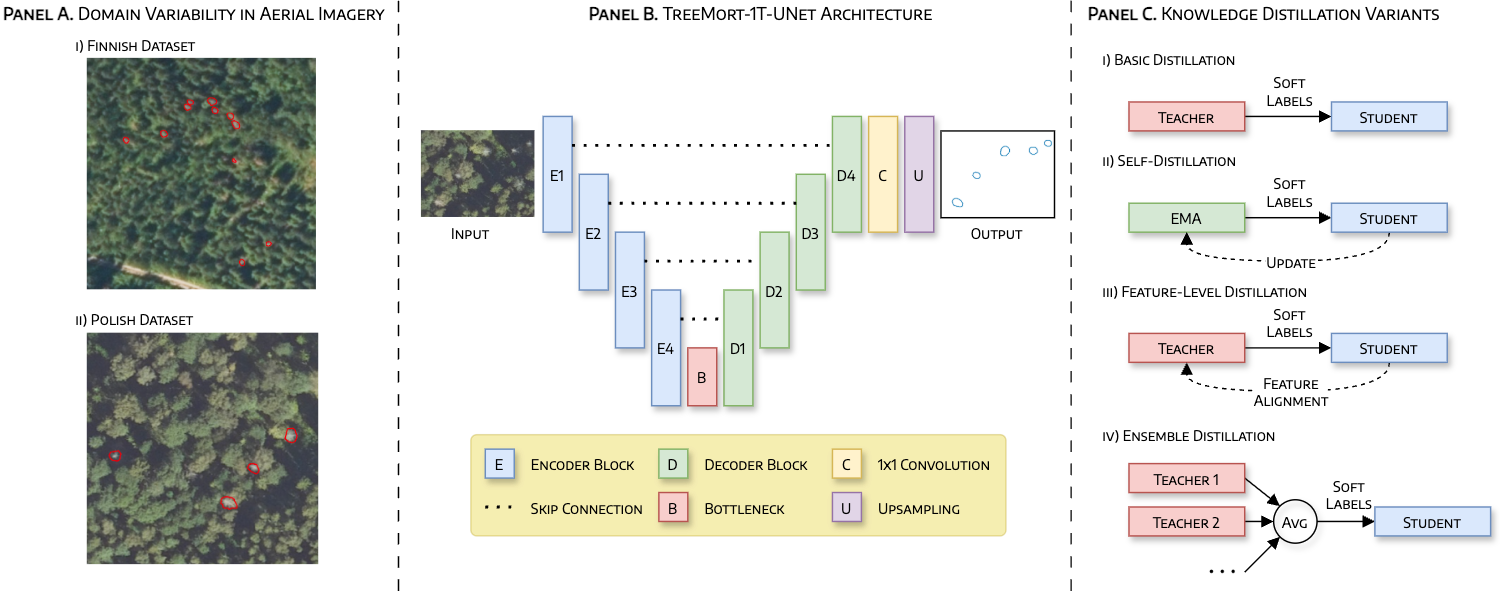
\includegraphics[width=\linewidth]{images/treemort-KD.png}
    \caption{
        Overview of the methodology for cross-domain dead tree detection in aerial imagery, presented in three panels. 
        Panel A illustrates the variability in the dataset, showcasing differences in forest density, tree species, and imaging conditions between Finnish and Polish aerial imagery, which pose significant challenges for domain adaptation in dead tree detection. 
        Panel B depicts the \oursone model architecture, highlighting its \textit{ResNet-34} encoder, self-attention-based decoder, and skip connections, designed for robust feature extraction and segmentation in multi-spectral aerial imagery. 
        Panel C presents the four KD variants: Basic, Self, Feature-level, and Ensemble, illustrating their mechanisms for transferring knowledge from teacher to student models to address domain variability and data scarcity.
    }
    \label{fig:overview}
\end{figure*}

\subsection{Dataset and Preprocessing}

The research uses high-resolution aerial imagery from four distinct regions: Finland, Poland, Germany, and Estonia, as summarized in Table~\ref{tbl:dataset}. The Finnish dataset, sourced from the National Land Survey of Finland~\citep{nlsf2024}, includes orthophotos captured between 2011 and 2023 with a true spatial resolution of 0.5 meters per pixel (resampled to 0.25 meters per pixel for this study), covering approximately 100 km$^2$ of diverse forest terrain. This dataset serves as the source domain for training the teacher model and contains approximately 17,500 manually annotated dead tree polygons (each consisting of a single dead tree), labeled by our collaborating forest health experts. The Polish dataset~\citep{gugik_orto}, used as the target domain for adaptation, comprises aerial imagery from Polish forests, which was standardized to the same resolution during preprocessing. Similarly, standing dead trees were manually annotated as polygons, around $9,700$ in total. The German dataset, sourced from Open NRW~\citep{open_nrw_2024}, and the Estonian dataset from the Estonian Land Board~\citep{maaamet_2024}, are used exclusively for evaluation to assess cross-domain generalization; they contain around 4,200 and 1,800 annotated dead trees, respectively, covering smaller areas with higher tree densities. The Estonian orthophotos feature resolutions of 0.20--0.40 m (general) and 0.10--0.16 m (settlements), with annual updates and CIR (color-infrared: NIR, red, green) bands suitable for forestry monitoring.

A multi-channel labeling scheme enhances detection and localization precision. The proposed scheme first employs a binary mask to signify dead tree presence. Then, a Gaussian heatmap is centered on tree centroids for accurate positioning, and a hybrid channel integrating the Signed Distance Transform with boundary details refines edge delineation. Given the large scale of the imagery, a patch-based approach segments images and labels into $256 \times 256$ pixel patches with a 128-pixel stride, ensuring 50\% overlap to maintain contextual integrity. A buffer mask excludes incomplete tree segments from each patch, guaranteeing that only fully represented trees contribute to training. These patches, stored in an HDF5 file, are organized by image and patch index, encapsulating multispectral RGB-NIR image data, label channels, and metadata such as tree counts and geographic coordinates.

Preprocessing normalizes pixel values to a $[0, 1]$ range using histogram truncation, clipping the top and bottom 2\% of values to mitigate outliers. Patches are uniformly sized via center cropping or padding, and an optional image processor adjusts the mean and standard deviation for multi-channel inputs. As data augmentation, we use random flips, rotations, brightness and contrast shifts, multiplicative noise, and gamma correction, which enhances model robustness by simulating varied imaging conditions. To counter class imbalance, where most patches lack dead trees, we have followed a balanced sampling approach ensuring equitable selection of patches with and without dead trees during training.

\begin{table*}[t!]
    \def\arraystretch{1.1}
    \centering
    \footnotesize
    \caption{Overview of datasets and key attributes used for model training and evaluation. Germany and Estonia are evaluation-only datasets.}
    \begin{adjustbox}{max width=\textwidth}
    \begin{tabular}{llcccc}
    \toprule
    ~ & 
    \textsc{\shortstack{Attribute}} & 
    \textsc{\shortstack{Finland}} & 
    \textsc{\shortstack{Poland}} & 
    \textsc{\shortstack{Germany}} & 
    \textsc{\shortstack{Estonia}} \\
    \midrule
    \multicolumn{6}{l}{\texttt{Common Acquisition Parameters}} \\
    & Spectral Bands & \multicolumn{4}{c}{RGB, NIR} \\
    & Patch Size & \multicolumn{4}{c}{$256 \times 256$ px} \\
    & Patch Overlap & \multicolumn{4}{c}{50\%} \\
    \midrule
    \multicolumn{6}{l}{\texttt{Image and Annotation Statistics}} \\
    & Spatial Resolution & 0.25 m & 0.25 m & 0.10 m & 0.25 m \\
    & Image Count & 126 & 166 & 30 & 15 \\
    & Area (km\textsuperscript{2}) & 98.49 & 33.15 & 7.68 & 3.99 \\
    & Acquisition Years & 2011, 2013--17, 2019, 2022--23 & 2021--22 & 2021--22 & 2022--23 \\
    & Dead Trees (annotated) & 22,772 & 10,205 & 4,188 & 2,922 \\
    & Avg. Dead Tree Density (/ha) & 2.31 & 3.08 & 5.46 & 7.33 \\
    \midrule
    \multicolumn{6}{l}{\texttt{Patch-Level Dataset Partitions}} \\
    & Patch Count & 87,458 & 17,648 & 7,264 & 3,128 \\
    & Labeled Trees & 624,966 & 27,087 & 14,616 & 4,915 \\
    & Train / Val / Test Trees & 454k / 127k / 43k & 16.0k / 8.3k / 2.8k & -- & -- \\
    \bottomrule
    \end{tabular}
    \end{adjustbox}
\label{tbl:dataset}
\end{table*}

\subsection{Model Architecture}

Our proposed model, \oursone (Tree Mortality 1-Task U-Net), is an adaptation of the \oursthree  (Tree Mortality 3-Task U-Net) architecture originally introduced in~\citep{rahman2025dual} for multi-task learning with three output channels, reconfigured here for binary dead tree segmentation with a single output mask to streamline computational demands while retaining high accuracy in identifying dead trees from aerial imagery. The key distinction from \oursthree is the reduction from three task-specific output heads (mask, centroid heatmap, signed distance transform) to a single binary segmentation head; the encoder and decoder structure are otherwise identical. We do not claim \oursone as a novel architecture: it is adopted here solely as a controlled backbone, ensuring that all teacher and student models share the same capacity and structure so that performance differences can be attributed cleanly to the KD strategy rather than to architecture. Built on the U-Net framework, it employs a \textit{ResNet-34} encoder, pre-trained on \textit{ImageNet} and adapted for four-channel RGB-NIR inputs, paired with a decoder featuring self-attention mechanisms to capture long-range dependencies, enhancing segmentation precision, and skip connections to preserve critical spatial information. In our knowledge distillation setup, both the teacher and student models are instances of \oursone, sharing the same architecture to isolate the effects of knowledge distillation on cross-domain adaptation. The teacher model is trained on the Finnish dataset using a hybrid loss function combining binary cross-entropy and Dice loss, optimized with the Adam algorithm~\citep{kingma2014adam}. The student model, initialized with distinct weights, is trained on the Polish dataset, utilizing the teacher's knowledge to adapt to this target domain. Future studies could explore employing a smaller or shallower student model to optimize computational efficiency.

\subsection{Knowledge Distillation Variants}

Knowledge distillation (KD) is a technique designed to transfer knowledge from a pre-trained teacher model to a student model, optimizing performance while addressing challenges such as domain variability and limited labeled data. In this study, we apply four KD variants: Basic, Self, Feature-level, and Ensemble, to adapt the \oursone model from Finnish to Polish aerial imagery for dead tree detection. These variants are tailored to the unique demands of remote sensing, where spectral and structural differences across regions complicate model generalization. Below, we detail each variant's conceptual basis, mathematical formulation, and implementation specifics.

\begin{enumerate}
\item\textbf{Basic KD} trains the student model to balance two objectives: matching ground truth labels and mimicking the teacher's softened predictions. The total loss is a weighted combination of the standard cross-entropy loss ($\mathcal{L}_{\text{CE}}$) and the distillation loss ($\mathcal{L}_{\text{KD}}$):
\begin{align}
\mathcal{L} = \alpha \mathcal{L}_{\text{KD}} + (1 - \alpha) \mathcal{L}_{\text{CE}}.
\end{align}

Here, $\alpha$ increases linearly from 0.3 to 0.7 over training epochs, gradually shifting focus toward the teacher's guidance. The distillation loss employs temperature-scaled probabilities to capture the teacher's nuanced confidence:
\begin{align}
\mathcal{L}_{\text{KD}} = T^2 \cdot \text{BCE} \left( \sigma \left( \frac{\mathbf{z}_s}{T} \right), \sigma \left( \frac{\mathbf{z}_t}{T} \right) \right),
\end{align}
where $\mathbf{z}_s$ and $\mathbf{z}_t$ are the student and teacher logits, respectively, and $\sigma$ is the sigmoid function. The temperature $T$ decreases from 6.0 to 2.0, refining the knowledge transfer as training progresses. A confidence mask ($\sigma(\mathbf{z}_t / T) > 0.3$) ensures the loss focuses on reliable teacher predictions, addressing the uncertainty in aerial imagery where dead trees may be partially obscured or spectrally similar to healthy vegetation.

\item\textbf{Self-KD} extends Basic KD by using an \textit{exponential moving average (EMA)} of the student's weights as a dynamic teacher, denoted as $\theta_\text{EMA}$, eliminating the need for a separate pre-trained model. The EMA teacher parameters are updated as:
\begin{align}
\theta_{\text{EMA}}^{t+1} = \beta \theta_{\text{EMA}}^t + (1 - \beta) \theta_s^t,
\end{align}
where $\theta_s^t$ represents the student's current weights. This approach allows the student to iteratively refine its predictions, leveraging its own evolving knowledge. The loss function mirrors that of Basic KD, with $\mathcal{L}_{\text{KD}}$ computed between the student's logits and those of the EMA teacher. The high decay rate $\beta = 0.999$ ensures stability, gradually incorporating the student's updates while maintaining a consistent reference point. This is a critical feature for the dead tree detection task, where domain-specific patterns must be learned incrementally.

\item\textbf{Feature-level KD} enhances knowledge transfer by aligning intermediate feature representations between the student and teacher models. The total loss incorporates a feature alignment term alongside the standard and distillation losses:
\begin{align}
\mathcal{L} = \mathcal{L}_{\text{CE}} + \alpha \mathcal{L}_{\text{KD}} + \lambda \mathcal{L}_{\text{feat}},
\end{align}
where $\alpha = 0.5$ and $\lambda = 1$. The feature loss $\mathcal{L}_{\text{feat}}$ combines mean squared error (MSE) and cosine similarity to align normalized feature maps from corresponding encoder layers:
\begin{align}
\mathcal{L}_{\text{feat}} = \sum_{i} w_i \Bigg( 
    \frac{1}{2} \, \text{MSE}(\hat{\mathbf{F}}_s^i, \hat{\mathbf{F}}_t^i) 
    + \frac{1}{2} \left(1 - \cos(\mathbf{F}_s^i, \mathbf{F}_t^i)\right) 
\Bigg), \notag
\end{align}
where $w_i = 1.0$ and $\hat{\mathbf{F}}^i$ denotes $\ell^2$-normalized features from the student ($\mathbf{F}_s^i$) and teacher ($\mathbf{F}_t^i$). This dual alignment, capturing both magnitude (via MSE) and direction (via cosine similarity), is particularly effective for aerial imagery, where spatial patterns and textures are crucial for distinguishing dead trees from healthy vegetation.

\item\textbf{Ensemble KD} improves robustness by aggregating predictions from multiple teacher models. The ensemble logits are computed as the mean of individual teacher logits:
\begin{align}
\mathbf{z}_{\text{ens}} = \frac{1}{M} \sum_{m=1}^{M} \mathbf{z}_{t_m},
\end{align}
where $\mathbf{z}_{t_m}$ is the logit from the $m$-th teacher, and $M$ is the number of teachers. The student's distillation loss targets $\mathbf{z}_{\text{ens}}$, following the same temperature scaling and confidence weighting as Basic KD. This approach leverages the diversity of teacher models to provide a more generalized target, which is advantageous in the context of forest ecosystems that exhibit significant variability across regions.
\end{enumerate}

In summary, the four KD variants offer complementary strategies for knowledge transfer, each addressing specific challenges in dead tree detection. Basic KD provides a balanced foundation, Self-KD enables iterative self-improvement, \textit{Feature-level KD} enhances spatial feature alignment, and Ensemble KD leverages multiple teachers for robustness. Together, these methods optimize the student model's performance, ensuring it is both computationally efficient and capable of generalizing across diverse aerial imagery datasets.

\subsection{Experimental Setup}

All experiments were conducted using the \oursone architecture with a ResNet-34 encoder, implemented in PyTorch. The teacher model was pre-trained on the Finnish source domain dataset for 100 epochs with early stopping (patience of 10 epochs) using the Adam optimizer (learning rate $1 \times 10^{-4}$, weight decay $1 \times 10^{-4}$), batch size 8, and a hybrid loss combining binary cross-entropy (BCE) and Dice for segmentation. Adaptation to the Polish target domain involved fine-tuning and KD variants on an 70/20/10 train/val/test split, with balanced sampling to address class imbalance (e.g., equal patches with/without dead trees).

For KD variants, the student model mirrored the teacher's architecture. Training used the same optimizer, batch size, and epochs per variant. Data augmentation (random flip, rotation, brightness, contrast, multiplicative noise, gamma correction) was applied during training. Evaluations on German and Estonian datasets were zero-shot (no training, direct inference).

As a domain adaptation baseline, we implement DANN~\citep{ganin2016domain}. A gradient reversal layer is applied to the bottleneck features (ResNet-34 layer4, 512 channels) feeding a two-layer domain discriminator. The gradient reversal strength follows $\lambda_{\text{GRL}} = 2/(1+\exp(-10p))-1$, where $p$ increases from 0 to 1 over training, with a domain loss weight $\lambda_{\text{DANN}}=0.1$. Training interleaves batches from the Finnish source domain and the target country (Finland = domain~0, target = domain~1).

KD hyperparameter choices follow established practice~\citep{hinton2015distilling,furlanello2018born}. The temperature schedule ($T$: $6.0\!\to\!2.0$) transfers soft uncertainty information at higher temperatures early in training, then sharpens student predictions as the loss stabilizes — consistent with the Born-Again-Network curriculum~\citep{furlanello2018born}. The $\alpha$ schedule ($0.3\!\to\!0.7$) progressively shifts emphasis from ground-truth supervision to teacher guidance as the student converges~\citep{hinton2015distilling}. The EMA decay $\beta=0.999$ in Self KD follows the mean-teacher convention for stable pseudo-target generation.

Key metrics include Tree IoU (IoU-matched instance-level intersection over union), Centroid Precision/Recall/F1 (distance-based, 5-pixel matching radius), and Tree TP/FP/FN counts. Representational analyses use penultimate layer features, with cosine/CKA/SSIM averaged over 1,000 subsampled patches per domain. Linear probing trains logistic regression (scikit-learn, default params) on frozen features for binary dead tree prediction. All runs used AMD MI250X GPUs (8 GPUs on LUMI HPC); inference $<$1 min per dataset. Code available upon acceptance.

\section{Results}
\label{sec:results}

In this section, we present the performance evaluation of our proposed KD strategies for cross-domain dead tree detection. We compare fine-tuning, DANN, and four KD variants on adaptation to the Polish target domain, cross-domain generalization across Germany and Estonia, data efficiency under limited annotations, and an ablation study on Feature-level KD components. Representational similarity analyses (cosine, CKA, SSIM, t-SNE, linear probing) assess domain invariance. All experiments use the same \textit{ResNet-34} U-Net architecture for teacher and student, ensuring that performance differences reflect training strategies rather than architectural choices.

\subsection{Performance on Target Domain}

We evaluate the fine-tuning baseline, DANN, and four KD variants on the Polish test set (4,521 ground-truth trees), with full details in Table~\ref{tbl:metrics}. Fine-tuning achieves Tree IoU of 0.216 (CI: 0.204--0.228) and centroid F1-score of 0.667, but leaves 2,105 trees undetected (Tree FN) due to domain mismatch. DANN improves on fine-tuning (Tree IoU 0.242; Tree TP 2,747; centroid F1 0.702), demonstrating that adversarial feature alignment provides measurable but modest gains.

All four KD variants substantially outperform both baselines. Self KD achieves the highest Tree IoU (0.277; CI: 0.263--0.290), while Basic KD achieves the best centroid precision (0.713) and fewest false positive detections (Tree FP 1,811). Ensemble KD obtains the highest centroid recall (0.800) and fewest missed trees (Tree FN 1,348). The 28\% improvement in Tree IoU from fine-tuning (0.216) to Self KD (0.277) underscores the value of teacher-guided transfer over supervised fine-tuning alone.

\begin{table*}[!t]
    \def\arraystretch{1.1}
    \centering
    \footnotesize
    \caption{Performance on the Polish target domain (4,521 ground-truth trees). Centroid-based metrics use a 5-pixel matching radius; Tree TP/FP/FN use IoU-matched assignments. The best is \textbf{bold}; second best is \underline{underlined}. Tree IoU brackets are 95\% confidence intervals.}
    \begin{adjustbox}{max width=\textwidth}
    \begin{tabular}{lccccccc}
    \toprule
    \textsc{\textbf{Method}} &
    \textsc{\textbf{\shortstack{Tree\\IoU}}} &
    \textsc{\textbf{\shortstack{Cent.\\Prec.}}} &
    \textsc{\textbf{\shortstack{Cent.\\Recall}}} &
    \textsc{\textbf{\shortstack{Cent.\\F1}}} &
    \textsc{\textbf{Tree TP}} &
    \textsc{\textbf{Tree FP}} &
    \textsc{\textbf{Tree FN}} \\
    \midrule

    Fine-tuned &
    0.216 [0.204--0.228]
    & 0.677 & 0.658 & 0.667
    & 2416 & 1977 & 2105 \\

    DANN~\citep{ganin2016domain} &
    0.242 [0.230--0.255]
    & 0.687 & 0.718 & 0.702
    & 2747 & 1978 & 1774 \\

    \midrule

    Basic KD &
    \underline{0.276} [0.263--0.289]
    & \textbf{0.713} & 0.779 & \textbf{0.744}
    & 3130 & \textbf{1811} & \underline{1391} \\

    Self KD &
    \textbf{0.277} [0.263--0.290]
    & 0.659 & \underline{0.796} & 0.721
    & \underline{3160} & 2298 & 1361 \\

    \textit{Feature-level KD} &
    0.263 [0.249--0.277]
    & 0.665 & 0.790 & \underline{0.722}
    & 3087 & 2284 & 1434 \\

    Ensemble KD &
    0.275 [0.262--0.288]
    & \underline{0.666} & \textbf{0.800} & 0.727
    & \textbf{3173} & \underline{2257} & \textbf{1348} \\

    \bottomrule
    \end{tabular}
    \end{adjustbox}
\label{tbl:metrics}
\end{table*}

These results reveal complementary operating points: Self KD maximizes Tree IoU; Basic KD offers the best centroid precision and fewest false positives; Ensemble KD yields the highest centroid recall and fewest misses. For precision-critical forestry applications where spurious detections trigger costly field visits, Basic KD's low false positive count (1,811 Tree FP vs.\ 1,977 for fine-tuning and 1,978 for DANN) represents a meaningful operational advantage. For visual reference, Figure~\ref{fig:samples} presents sample aerial images with ground truth annotations and model predictions, illustrating how KD-adapted models detect dead trees with improved spatial accuracy compared to fine-tuning.

\begin{figure*}[!t]
    \centering
    \subfloat{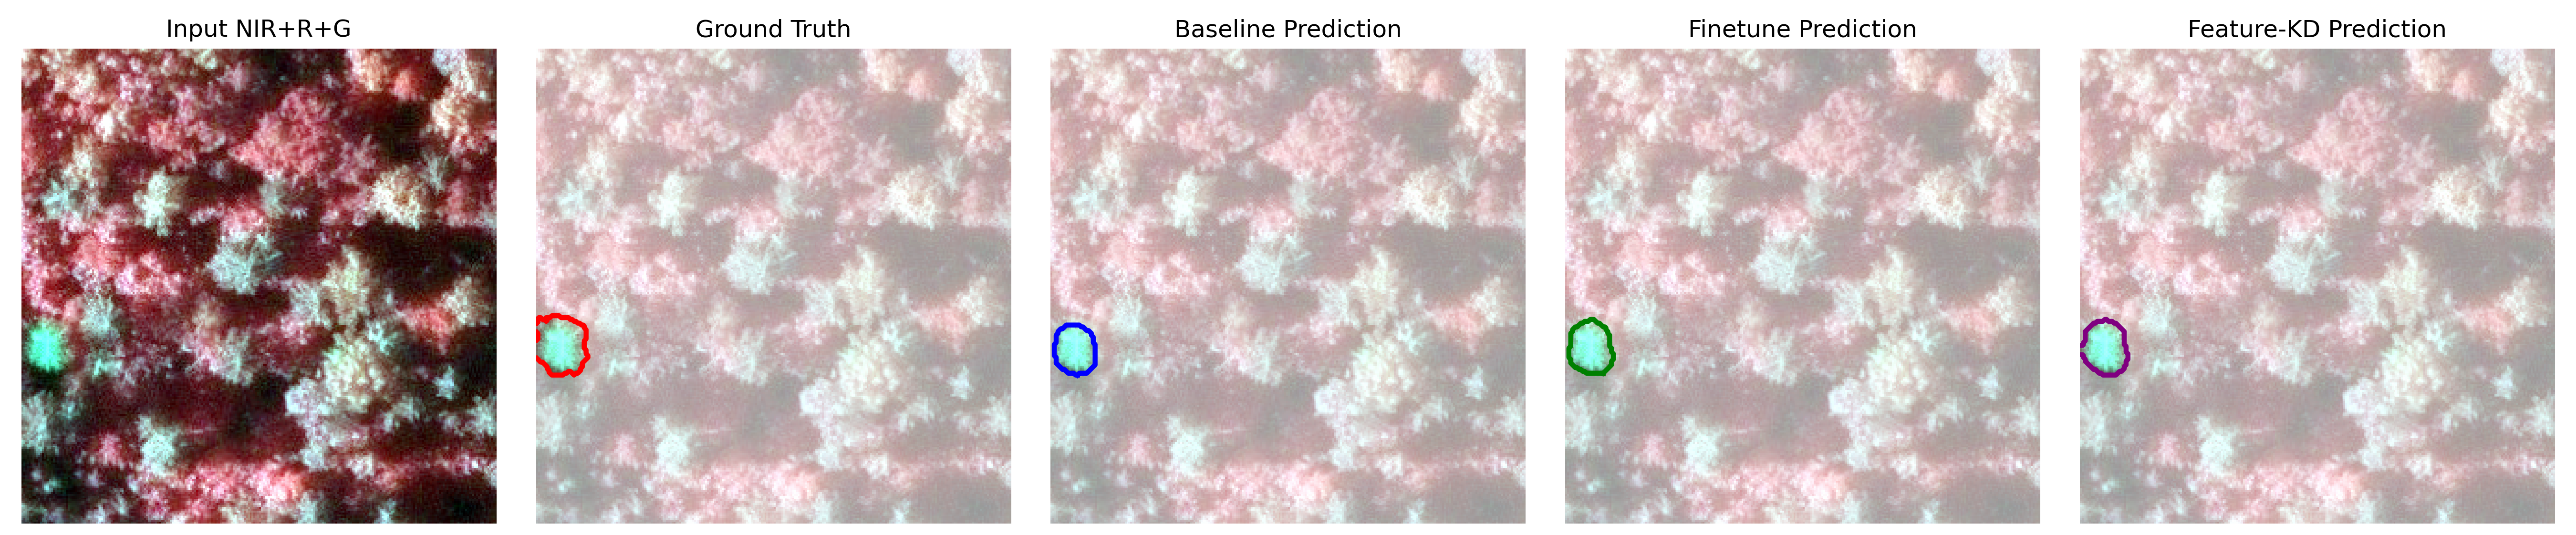
\includegraphics[width=\linewidth]{images/s1.png} \label{subfig:sample1}}
    
    \subfloat{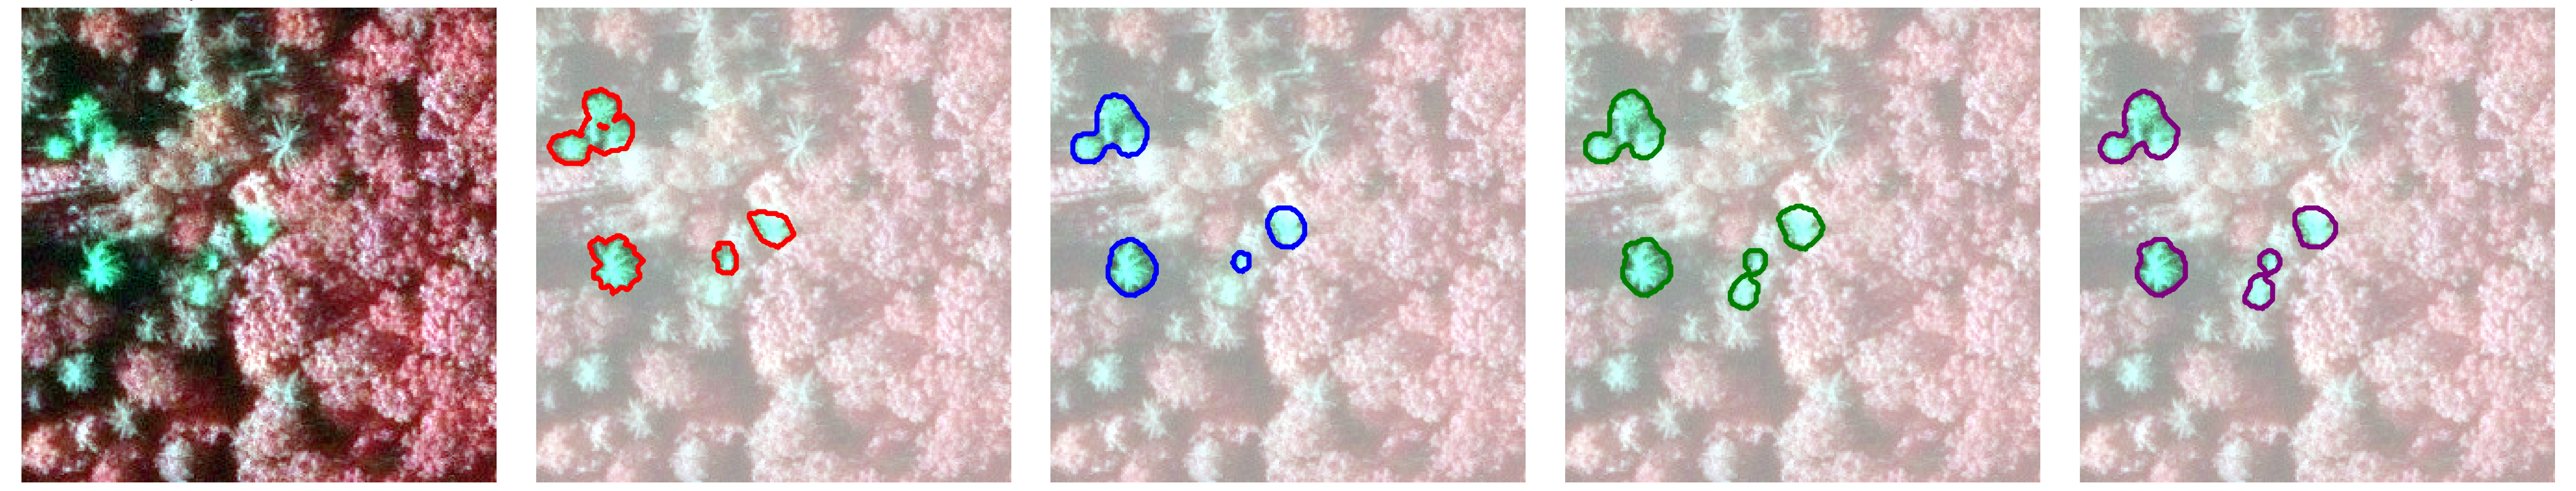
\includegraphics[width=\linewidth]{images/s2.png} \label{subfig:sample2}}
    
    \subfloat{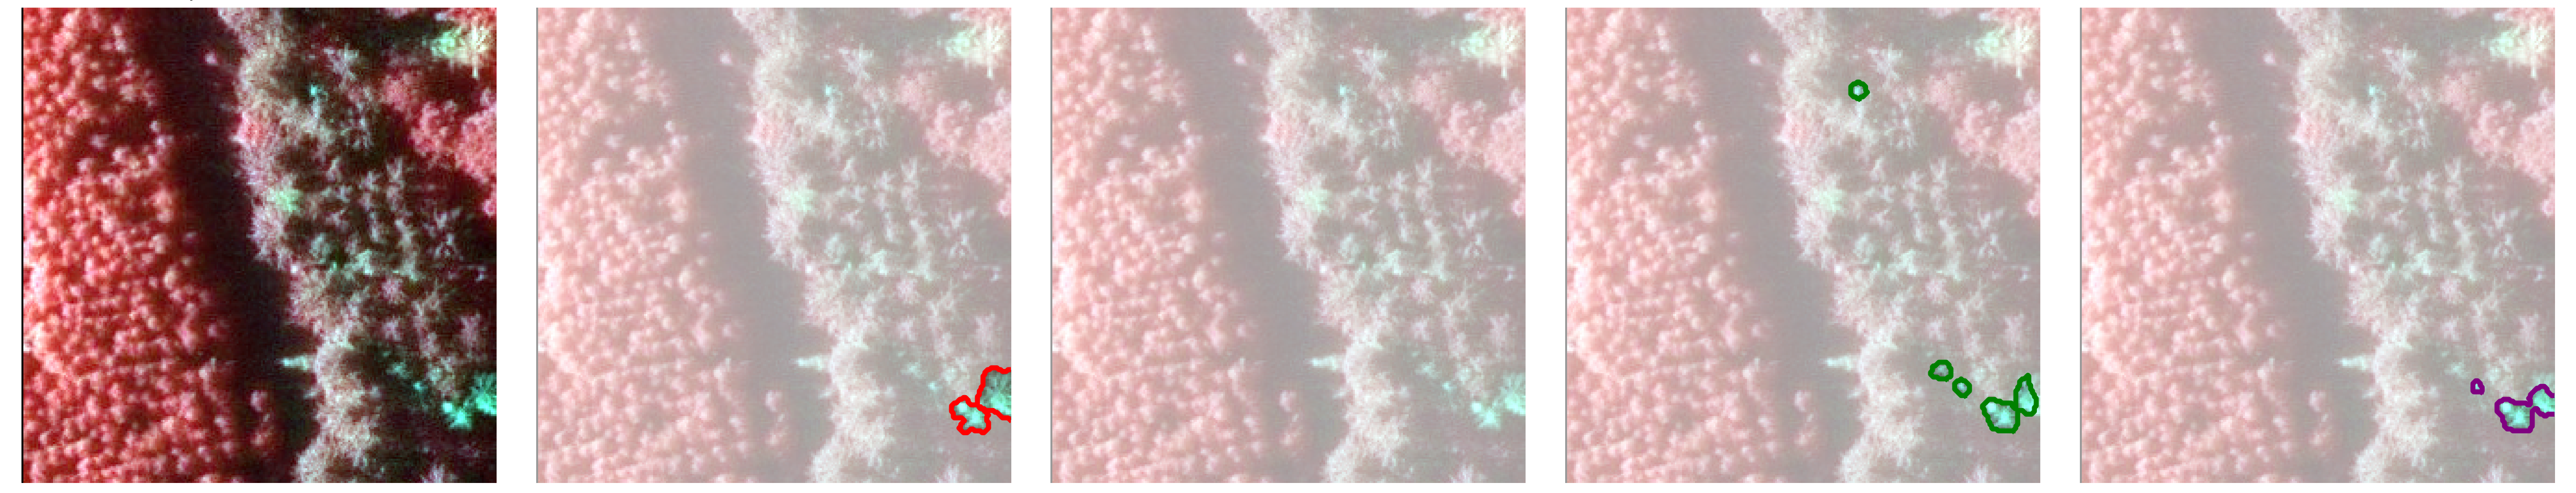
\includegraphics[width=\linewidth]{images/s3.png} \label{subfig:sample3}}
    
    \subfloat{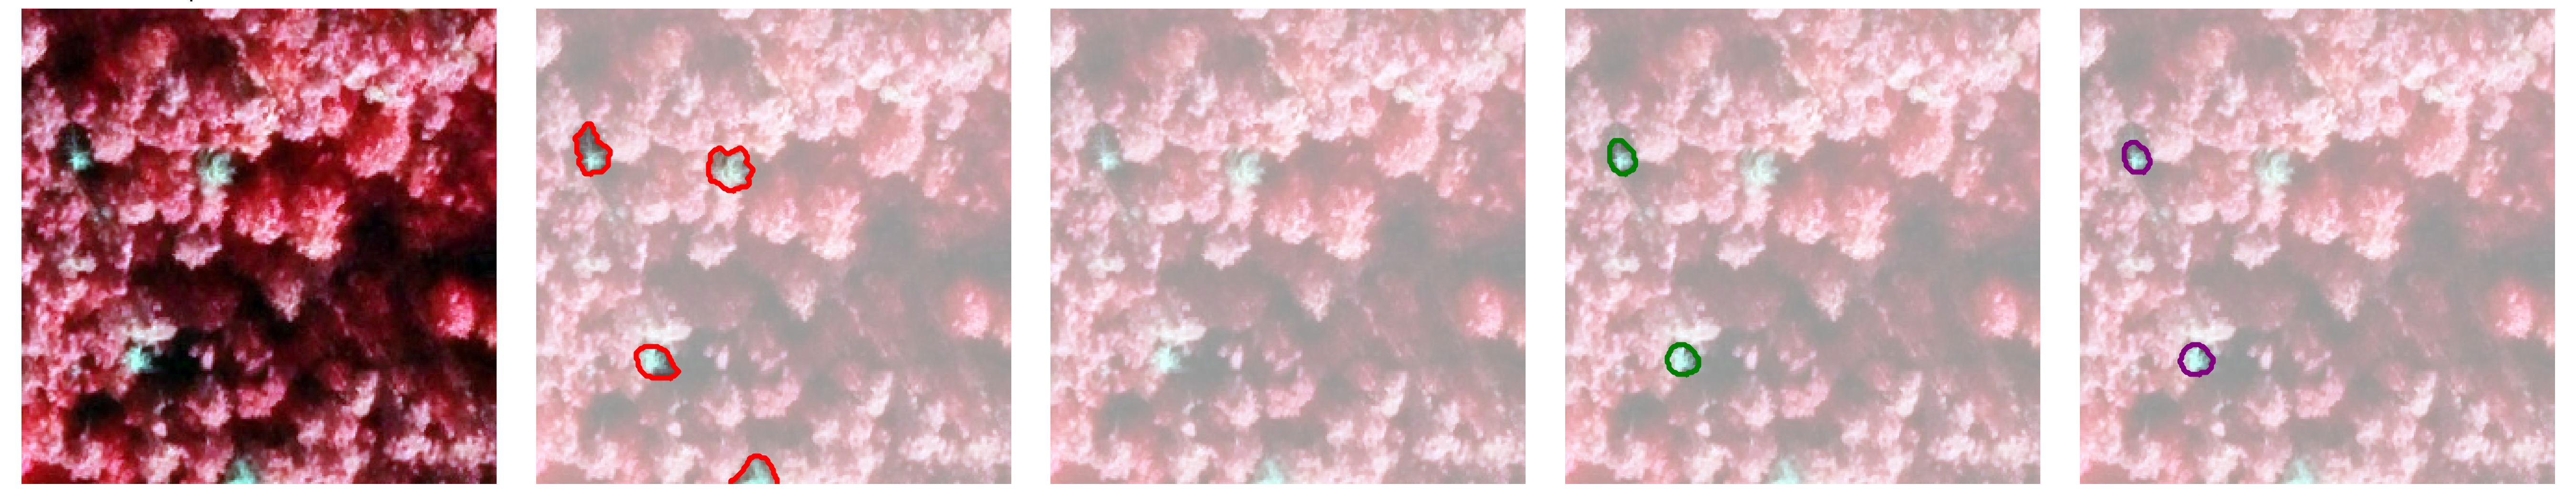
\includegraphics[width=\linewidth]{images/s4.png} \label{subfig:sample4}}
    
    % \subfloat{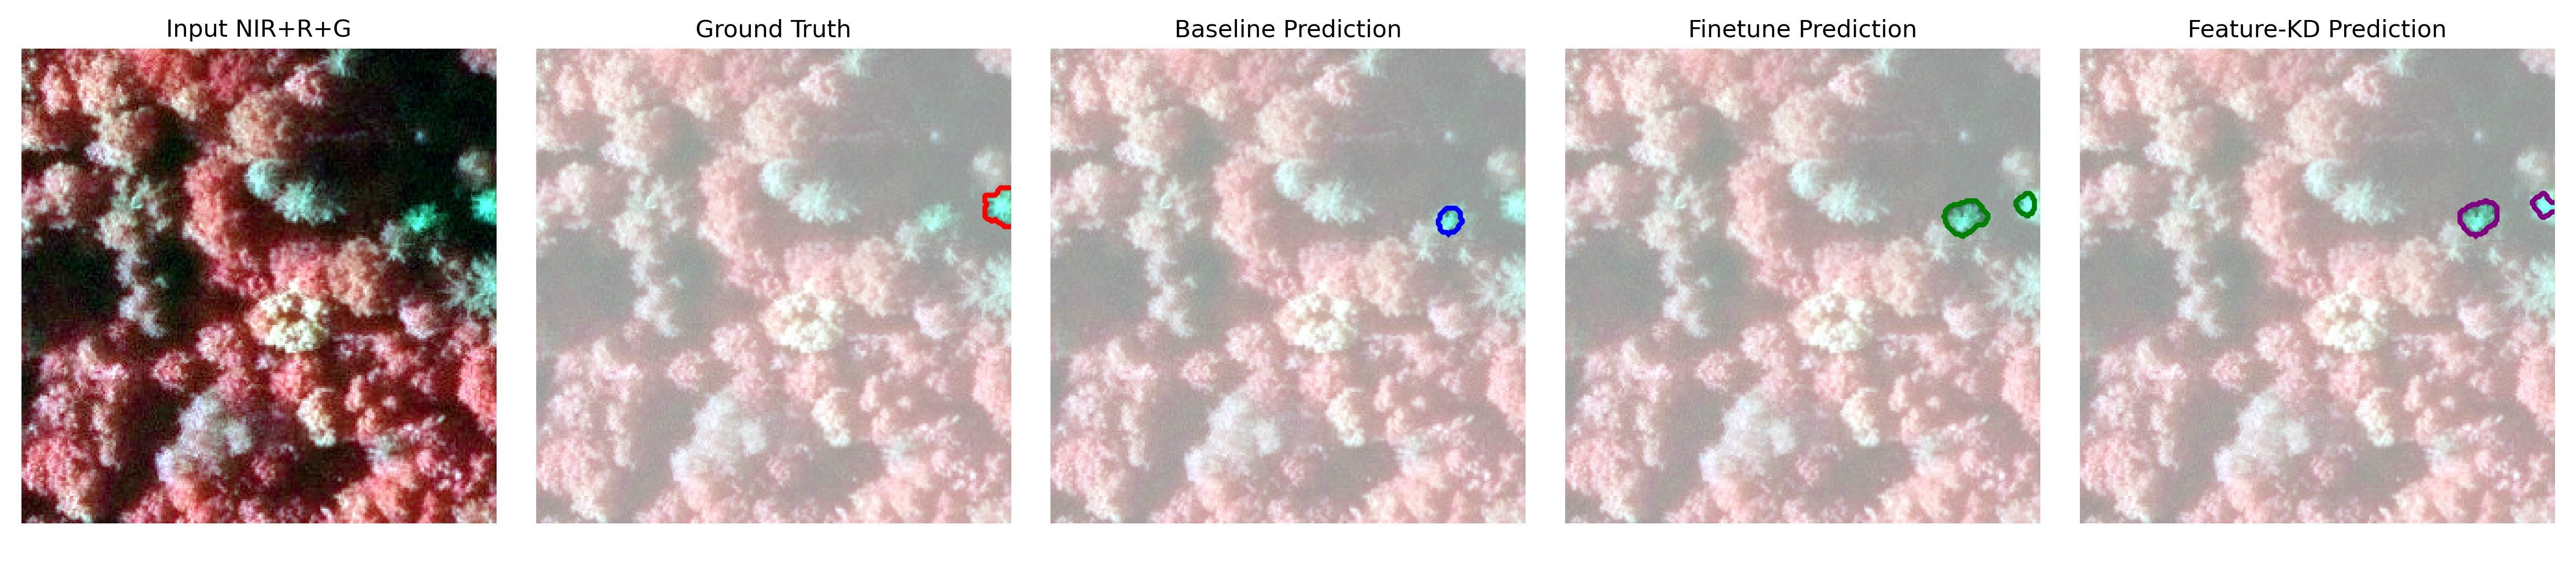
\includegraphics[width=\linewidth]{images/s5.png} \label{subfig:sample5}}
    
    % \subfloat{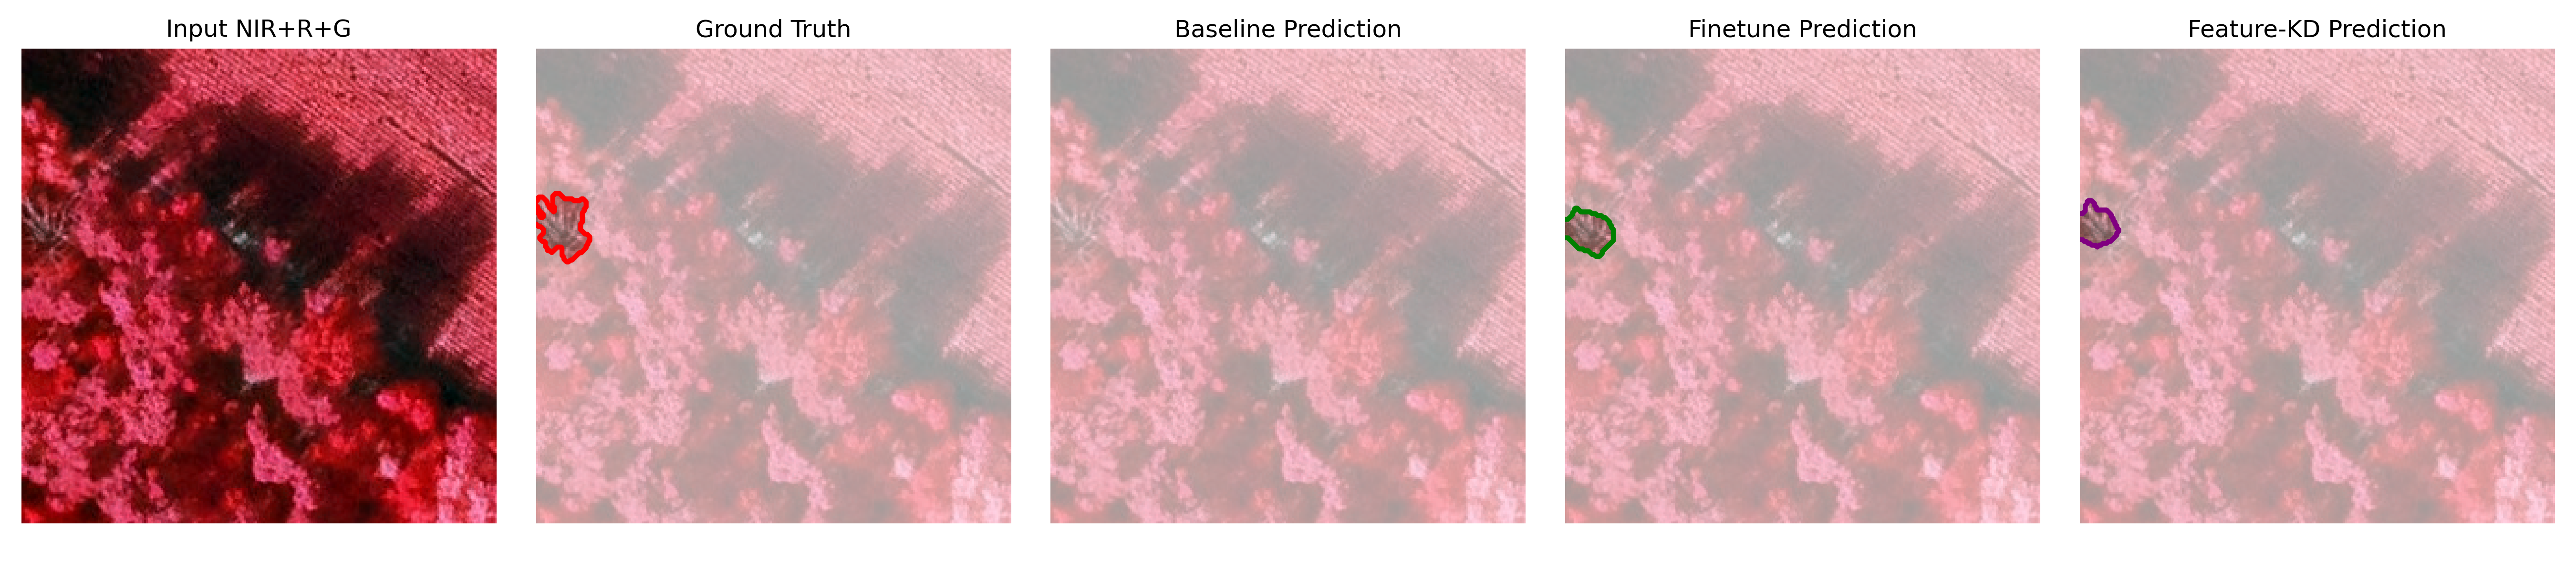
\includegraphics[width=\linewidth]{images/s6.png} \label{subfig:sample6}}
    
    \caption{Visual comparison of ground truth annotations and model predictions for standing dead tree segmentation. Columns show (from left to right): (1) input composite image (NIR, red, green bands), (2) ground truth annotations (red), (3) baseline model prediction (blue), (4) fine-tuned student model prediction (green), and (5) feature-based knowledge distillation (KD) student model prediction (purple). Mask overlays are semi-transparent with corresponding contours to highlight detected regions.}

    \label{fig:samples}
\end{figure*}

\subsection{Cross-Domain Generalization}

We evaluate all methods on Poland (4,521 test trees), Germany (79 test trees), and Estonia (962 test trees) using models trained on Finland (teacher Tree IoU: 0.448), with results in Table~\ref{tbl:cross_domain}. Zero-shot transfer --- applying the Finnish teacher directly without any adaptation --- yields Tree IoU of 0.121 on Poland, 0.000 on Germany, and 0.219 on Estonia, establishing the adaptation gap that motivates all strategies below.

\begin{table}[!t]
    \def\arraystretch{1.1}
    \centering
    \footnotesize
    \caption{Cross-domain Tree IoU across three target countries. Teacher is trained on Finland (Tree IoU 0.448). Best per country is \textbf{bold}; second best is \underline{underlined}.}
    \begin{adjustbox}{max width=\columnwidth}
    \begin{tabular}{lccc}
    \toprule
    \textsc{\textbf{Method}} &
    \textsc{\textbf{Poland}} &
    \textsc{\textbf{Germany}} &
    \textsc{\textbf{Estonia}} \\
    \midrule
    Zero-shot (teacher)               & 0.121 & 0.000 & 0.219 \\
    Fine-tuned                        & 0.216 & 0.108 & 0.202 \\
    DANN~\citep{ganin2016domain}      & 0.242 & 0.083 & 0.205 \\
    \midrule
    Basic KD                          & \underline{0.276} & 0.302 & 0.226 \\
    Self KD                           & \textbf{0.277} & \textbf{0.328} & 0.233 \\
    \textit{Feature-level KD}         & 0.263 & 0.252 & \textbf{0.265} \\
    Ensemble KD                       & 0.275 & \underline{0.313} & \underline{0.255} \\
    \bottomrule
    \end{tabular}
    \end{adjustbox}
\label{tbl:cross_domain}
\end{table}

All four KD variants outperform both fine-tuning and DANN across all three countries. The gain is most pronounced for Germany, where zero-shot transfer yields Tree IoU of exactly 0.000 (the teacher detects no trees), yet Self KD recovers to 0.328 --- demonstrating that KD is not merely an incremental improvement but an essential mechanism when domain gaps are large enough to render the teacher completely non-functional. On Poland, all KD variants substantially exceed both the zero-shot baseline (0.121) and fine-tuning (0.216), with Self KD reaching 0.277 (2.3$\times$ zero-shot).

Estonia reveals a distinct regime: the zero-shot teacher achieves Tree IoU 0.219, which already exceeds fine-tuning (0.202) and DANN (0.205). This occurs because Estonia's boreal forest structure and CIR spectral bands are more similar to Finland than Poland's temperate forests are, so the Finnish teacher generalizes without adaptation. However, fine-tuning on Polish data degrades Estonia performance by shifting representations toward temperate-forest patterns. All KD variants improve over both zero-shot and fine-tuning on Estonia (Feature-level KD: 0.265), demonstrating that knowledge distillation preserves source-domain generalisation while still adapting to the target.

DANN underperforms fine-tuning on Germany (0.083 vs.\ 0.108), where the small test set (79 trees) and large resolution shift (0.10~m vs.\ 0.25~m) may prevent the gradient-reversal discriminator from converging. DANN provides only marginal gains on Poland (0.242) and Estonia (0.205), confirming that adversarial feature alignment is less effective than teacher-guided distillation across all conditions tested.

Self KD leads on Poland (0.277) and Germany (0.328) via its EMA-based self-improvement mechanism. Feature-level KD leads on Estonia (0.265) through multi-scale feature alignment that is particularly effective for CIR spectral conditions and high tree density. Ensemble KD provides consistent second-place performance on Germany (0.313) and Estonia (0.255), making it a reliable choice when the target domain is unknown in advance.

\subsection{Data Efficiency versus Data Scarcity}

We compare \textit{Fine-tuned} and \textit{Feature-level KD} using reduced amounts of Polish training data (100\%, 75\%, 50\%, and 25\%; see Table~\ref{tbl:data_analysis}). \textit{Feature-level KD} outperforms \textit{Fine-tuned} on Tree IoU at every data fraction, with an advantage of 0.040--0.047 across conditions. Notably, \textit{Feature-level KD} at 25\% data (Tree IoU 0.262) exceeds \textit{Fine-tuned} trained on the full dataset (0.231), demonstrating that teacher guidance compensates for annotation scarcity. \textit{Feature-level KD} also achieves higher Recall across all fractions (0.68--0.72 vs.\ 0.56--0.59), reflecting its ability to leverage Finnish teacher predictions to detect trees that a purely fine-tuned student misses. The absolute gap narrows only slightly from 100\% to 25\%, confirming that knowledge distillation retains its advantage even under severe data constraints.

\begin{table}[!t]
    \def\arraystretch{1.1}
    \centering
    \footnotesize
    \caption{Data efficiency analysis of \textit{Fine-tuned} and \textit{Feature-level KD} on the Polish test set under varying training data percentages. The best performer is marked by \textbf{bold text}.}
    \begin{adjustbox}{max width=0.8\columnwidth}
    \begin{tabular}{llcccccccccccc}
    \toprule
    ~ & \textsc{\textbf{Model}}
    & \textsc{\shortstack{Mean\\Tree IoU}}
    & \textsc{\shortstack{F1\\Score}}
    & \textsc{\shortstack{Prec.}}
    & \textsc{\shortstack{Recall}}
    & \textsc{\shortstack{TP}}
    & \textsc{\shortstack{FP}}
    & \textsc{\shortstack{FN}} \\
    
    \midrule
    
    \multicolumn{9}{l}{\texttt{100\%}} \\
    & \textit{Fine-tuned}        & 0.231 & 0.59 & \textbf{0.63} & 0.56 & 2545 & \textbf{1507} & \textbf{1976} \\
    & \textit{Feature-level KD}  & \textbf{0.274} & \textbf{0.64} & 0.59 & \textbf{0.70} & \textbf{3183} & 2224 & 1338 \\

    \midrule

    \multicolumn{9}{l}{\texttt{75\%}} \\
    & \textit{Fine-tuned}        & 0.228 & 0.58 & \textbf{0.57} & 0.59 & 2681 & \textbf{2055} & \textbf{1840} \\
    & \textit{Feature-level KD}  & \textbf{0.268} & \textbf{0.62} & 0.54 & \textbf{0.72} & \textbf{3269} & 2737 & 1252 \\

    \midrule

    \multicolumn{9}{l}{\texttt{50\%}} \\
    & \textit{Fine-tuned}        & 0.239 & 0.61 & \textbf{0.63} & 0.59 & 2676 & \textbf{1601} & \textbf{1845} \\
    & \textit{Feature-level KD}  & \textbf{0.270} & \textbf{0.64} & 0.61 & \textbf{0.68} & \textbf{3065} & 1923 & 1456 \\

    \midrule

    \multicolumn{9}{l}{\texttt{25\%}} \\
    & \textit{Fine-tuned}        & 0.221 & 0.58 & \textbf{0.57} & 0.59 & 2652 & \textbf{2017} & \textbf{1869} \\
    & \textit{Feature-level KD}  & \textbf{0.262} & \textbf{0.64} & 0.60 & \textbf{0.68} & \textbf{3078} & 2096 & 1443 \\

    \bottomrule
    \end{tabular}
    \end{adjustbox}
\label{tbl:data_analysis}
\end{table}

\subsection{Ablation Study of \textit{Feature-level KD} Components}

To evaluate the contribution of individual components in the proposed \textit{Feature-level KD}, we conducted an ablation study with three simplified variants: removing the feature alignment loss, disabling confidence-based weighting, and disabling foreground-background (FG-BG) weighting. These experiments use the original teacher configuration to isolate architectural effects; the updated teacher used in the main results further amplifies these contributions. Results (Table~\ref{tbl:ablation}) indicate that the complete KD setup achieved the highest F1-score and Mean Tree IoU, confirming the combined benefit of the strategies. Removing the feature loss led to the most pronounced degradation (F1: 0.48; IoU: 0.091), underscoring the critical role of aligning intermediate representations in maintaining performance. Omitting FG-BG weighting resulted in a notable drop in F1-score (0.49) and IoU (0.089), with a slight increase in Recall (0.78 vs. full 0.75), suggesting that emphasizing foreground pixels enhances detection robustness for small, sparse objects. Disabling confidence weighting similarly reduced F1-score (0.50) and IoU (0.090), with a minor Recall boost (0.78), indicating a marginal role in precision optimization. These findings affirm that each component contributes meaningfully to KD's success, with feature supervision being the most critical, followed by FG-BG weighting for balanced detection and recall performance.

\begin{table}[!t]
    \def\arraystretch{1.1}
    \centering
    \footnotesize
    \caption{Ablation study on Polish dataset.}
    \begin{adjustbox}{max width=0.7\columnwidth}
    \begin{tabular}{lccccc}
    \toprule
    \textsc{\textbf{Model}} 
    & \textsc{\shortstack{Mean\\Tree IoU}} 
    & \textsc{\shortstack{F1\\Score}} 
    & \textsc{\shortstack{Prec.}} 
    & \textsc{\shortstack{Recall}} \\
    
    \midrule

    \textit{Feature-level KD}   & 0.106 & 0.63 & 0.55 & 0.75 \\

    \midrule
    
    No Feature Loss             & 0.091 & 0.48 & 0.34 & 0.79 \\
    No Confidence Weighting     & 0.090 & 0.50 & 0.36 & 0.78 \\
    No FG-BG Weighting          & 0.089 & 0.49 & 0.35 & 0.78 \\

    \bottomrule
    \end{tabular}
    \end{adjustbox}
\label{tbl:ablation}
\end{table}

\subsection{Representational Similarity Analysis}

In this section, we analyze the representational similarities between the \textit{Baseline}, \textit{Fine-tuned}, and \textit{Feature-level KD} models using layer-wise metrics inspired by recent work on model convergence~\citep{ciernik2024objective}. Specifically, we compute mean cosine similarity (local, directional alignment), linear Centered Kernel Alignment (CKA; global, structural alignment), and Structural Similarity Index Measure (SSIM; perceptual structure) across the four encoder layers of the \textit{ResNet-34} backbone. These are evaluated on the Polish (target) and Finnish (source) datasets, focusing on pairwise comparisons: \textit{Baseline} vs. \textit{Fine-tuned}, \textit{Baseline} vs. \textit{Feature-level KD}, and \textit{Fine-tuned} vs. \textit{Feature-level KD} (on Polish only, emphasizing target adaptation). Additionally, we examine intra-model cosine similarity and SSIM across datasets (Finland vs. Poland) to quantify domain invariance within each model, apply t-SNE to visualize domain separation, and assess representation quality via linear probing (training a logistic regression classifier on frozen layer representations to predict dead tree presence, reporting accuracy (acc), F1-score (f1), and AUC (auc)).

Cross-dataset consistency, quantified via Pearson correlation \(\rho\) between flattened layer-wise similarities (following~\cite{ciernik2024objective}), is high for \textit{Baseline} pairs (\(\rho \approx 0.997\) for both cosine and CKA), indicating stable relative alignments. These results align with~\citep{ciernik2024objective}, where adaptation objectives drive consistency: \textit{Feature-level KD} (analogous to self-supervised objectives) yields more invariant representations than finetuning, explaining its superior cross-domain precision and reduced false positives (Table~\ref{tbl:metrics}).

\mypar{Inter-Model Representational Similarity}:
Inter-model similarities reveal how adaptations preserve or diverge from the \textit{Baseline} (Figure~\ref{fig:inter_model_sim}). Cosine similarities are high in early layers (0.94--0.999), reflecting shared low-level features (e.g., spectral textures), but decrease in deeper layers (0.73--0.99), where semantic adaptations occur. CKA shows similar trends but with greater divergence in Layer 4 (0.21--0.95), penalizing structural mismatches more severely. \textit{Feature-level KD} outperforms \textit{Fine-tuned} in alignment with the \textit{Baseline} on the target domain (e.g., CKA Layer 3: 0.903 vs. 0.897; Layer 4: 0.488 vs. 0.419), suggesting better retention of source knowledge via distillation.

\begin{figure}[!t]
    \centering
    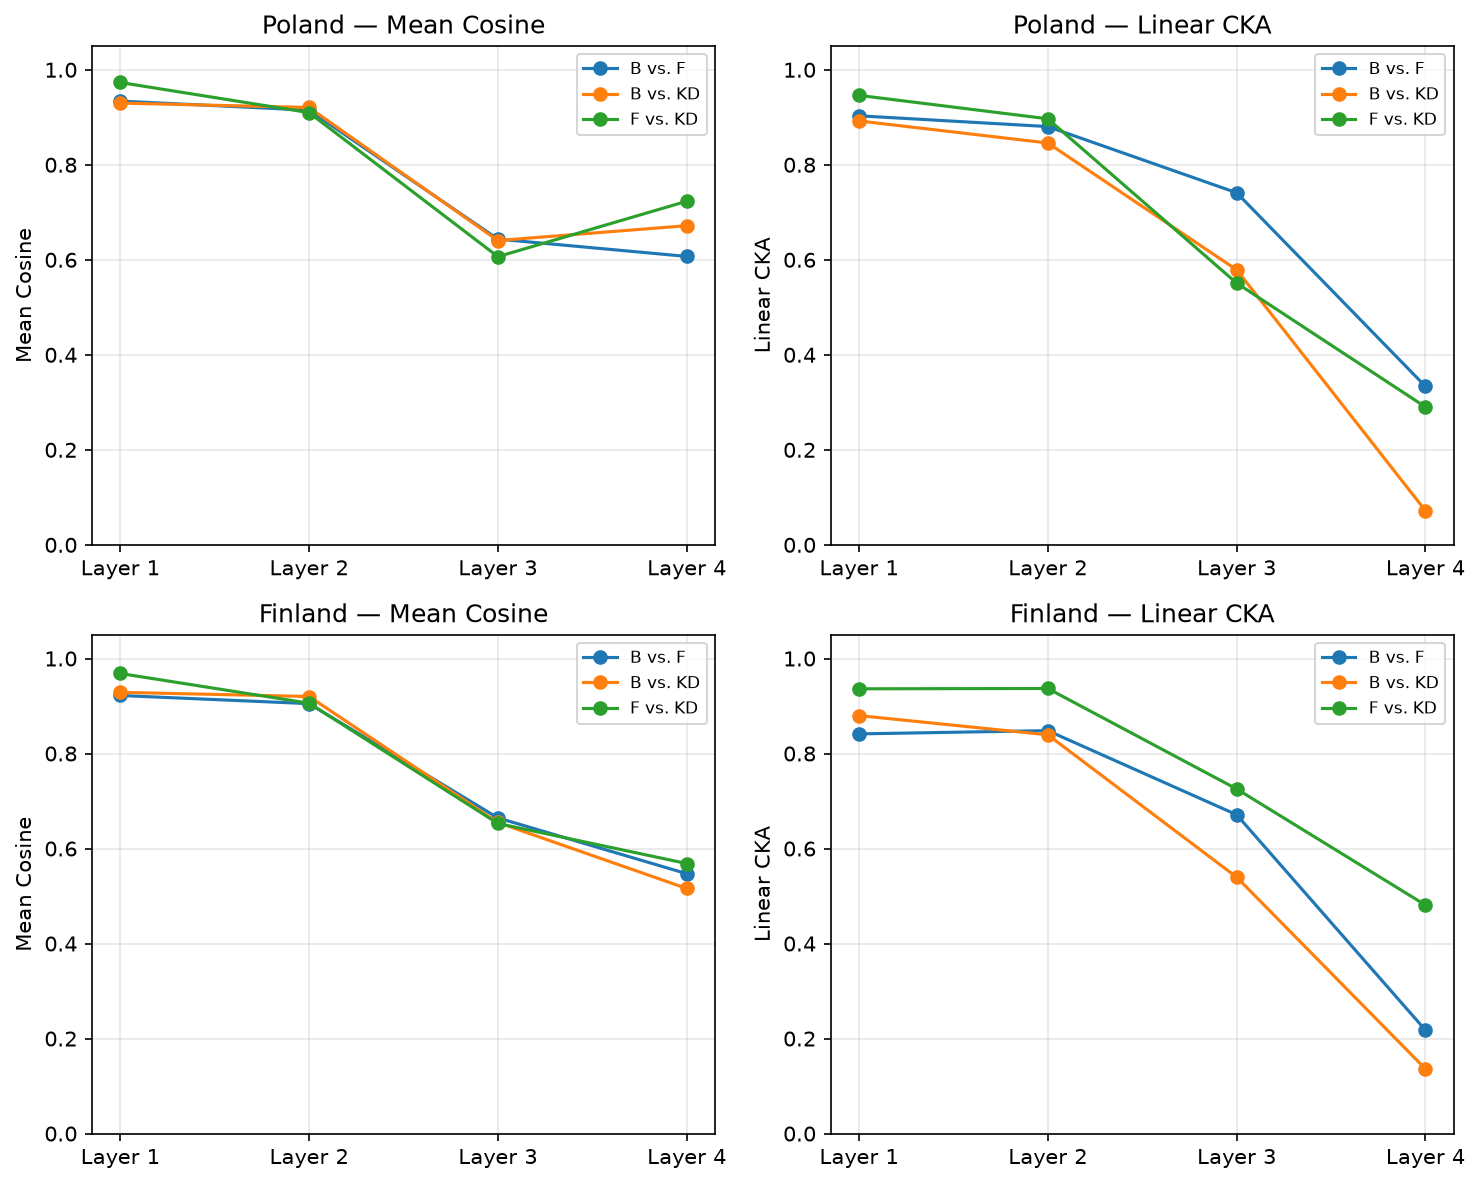
\includegraphics[width=\linewidth]{images/inter_model_similarity.png}
    \caption{Inter-model mean cosine and linear CKA similarities across layers for model pairs on Polish and Finnish datasets. Model pairs are abbreviated as: B vs. F (\textit{Baseline} vs. \textit{Fine-tuned}), B vs. KD (\textit{Baseline} vs. Feature-KD), and F vs. KD (\textit{Fine-tuned} vs. Feature-KD).}
    \label{fig:inter_model_sim}
\end{figure}

\mypar{Intra-Model Domain Invariance}:
Intra-model cosine similarities between representations on Finland and Poland (Table~\ref{fig:intra_cosine_ssim}) exhibit decreasing trends from Layer 1 to Layer 3 (0.92--0.93 to 0.54--0.56), indicating progressive domain shift, with partial recovery in Layer 4 (0.56--0.67). The \textit{Baseline} shows the lowest deep-layer consistency (Layer 3: 0.542; Layer 4: 0.671), reflecting raw boreal-to-temperate differences. \textit{Fine-tuned} and \textit{Feature-level KD} improve invariance, with \textit{Feature-level KD} slightly superior in Layers 2--4 (e.g., Layer 4: 0.573 vs. 0.561). SSIM further quantifies structural invariance on Poland, showing low values overall with increases from Layer 1/2 (0.028) to Layer 3 (0.157--0.172) before dropping in Layer 4 (0.05--0.10). The \textit{Baseline} exhibits higher SSIM in deeper layers (Layer 3: 0.157; Layer 4: 0.103), while \textit{Feature-level KD} slightly outperforms \textit{Fine-tuned} in Layer 4 (0.053 vs. 0.051), preserving marginally more perceptual details across domains.

\begin{figure}[!t]
    \centering
    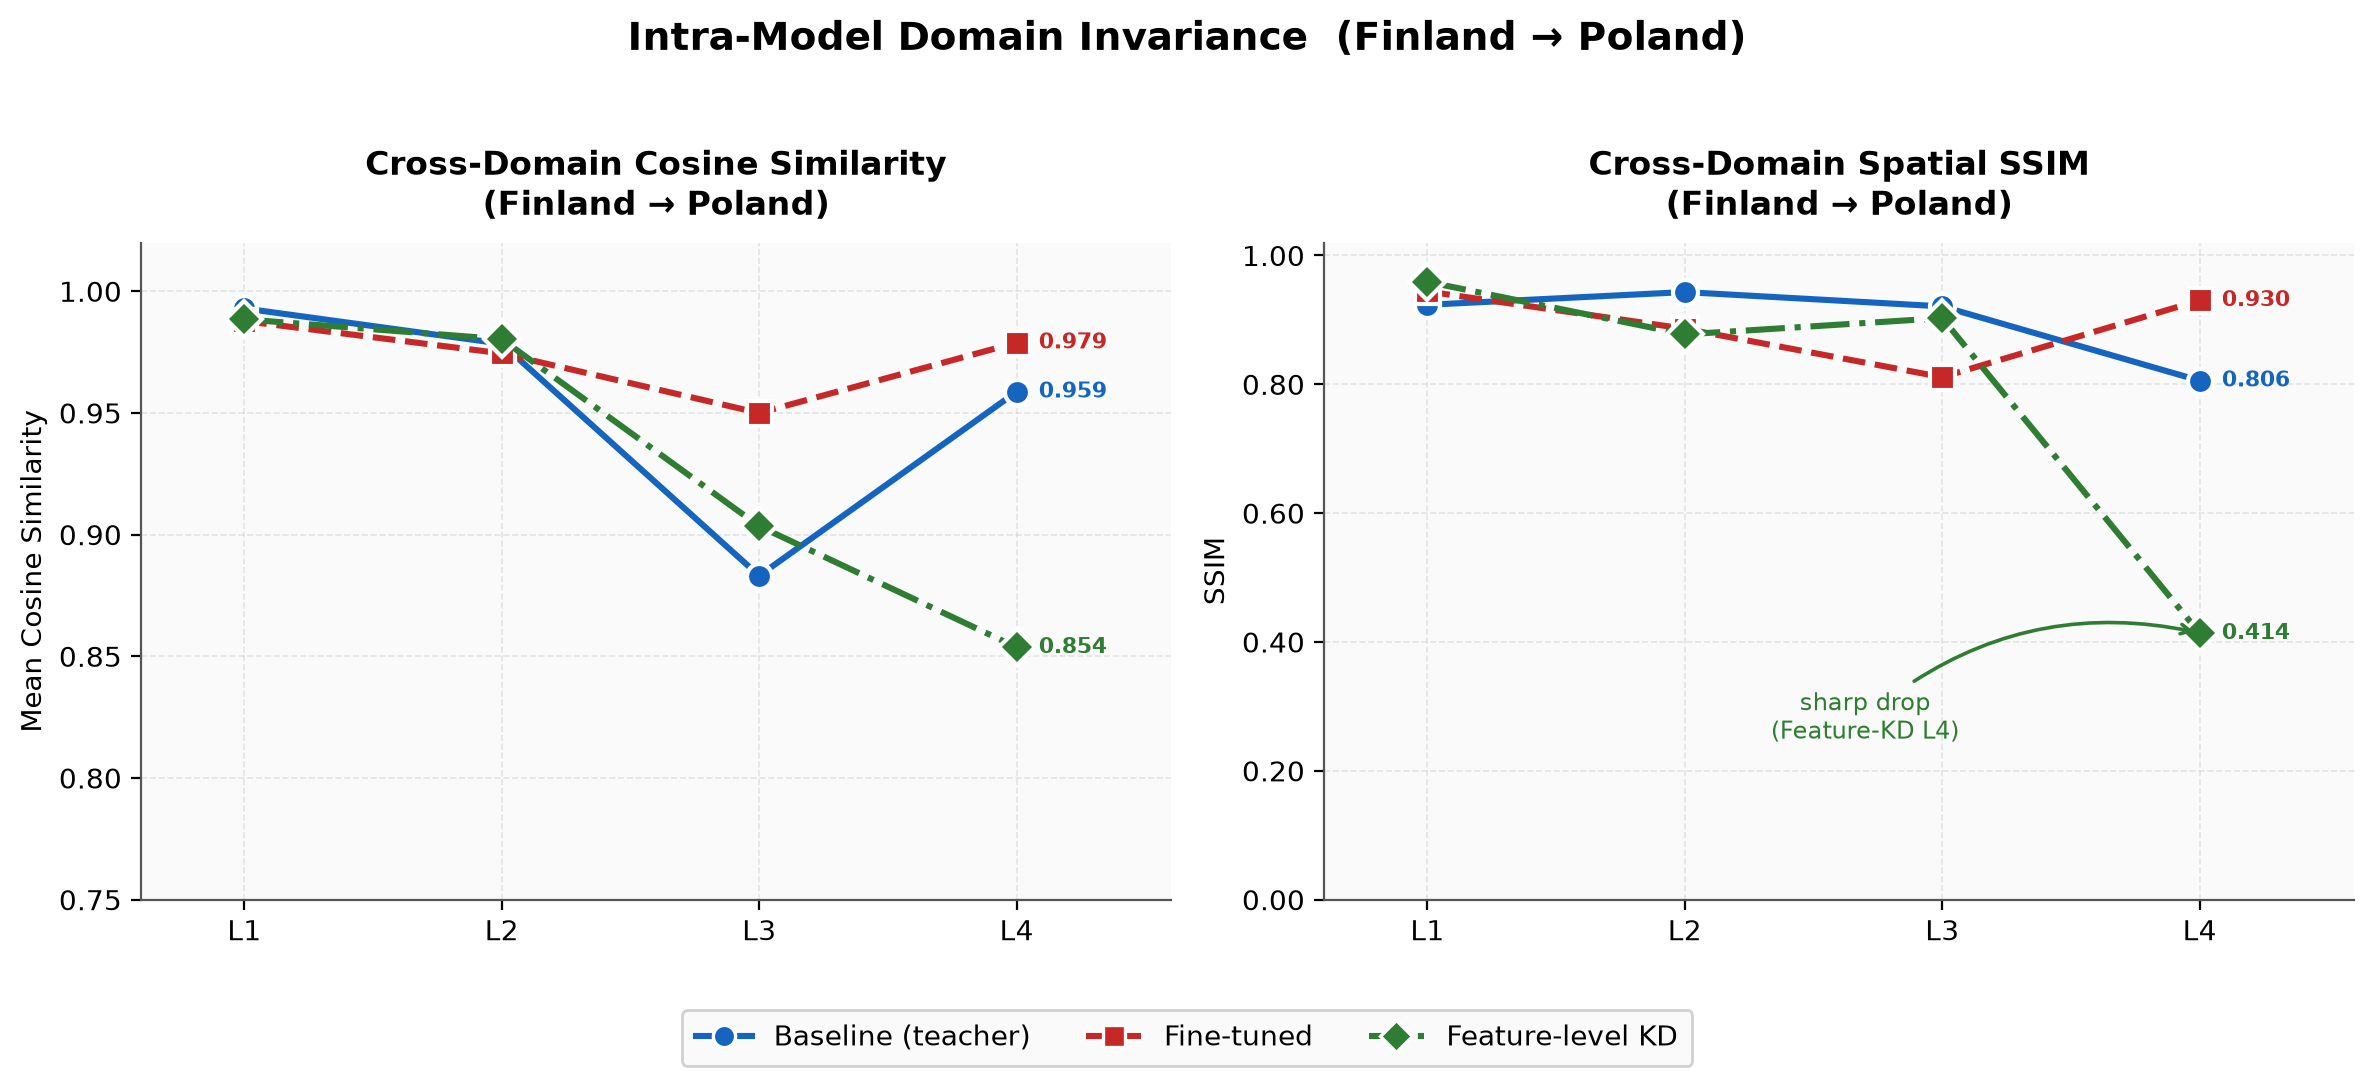
\includegraphics[width=\linewidth]{images/intra_model_similarity.png}
    \caption{Intra-model mean cosine similarity and SSIM across layers between Finland and Poland datasets.}
    \label{fig:intra_cosine_ssim}
\end{figure}

\mypar{Visualization via t-SNE}:
We apply t-SNE to concatenated representations from Finland and Poland for each model pair, computing cluster metrics: Silhouette Score (separation/cohesion), Centroid Distance (domain shift), Compactness (intra-domain variance), and Domain Overlap Ratio (mixing). Table~\ref{tbl:tsne_metrics} summarizes these, with corresponding scatterplots in Figure~\ref{fig:tsne_scatterplots}. On Poland, \textit{Fine-tuned} vs. \textit{Feature-level KD} shows low Silhouette (0.003) and Centroid Distance (2.78), with high Overlap (0.491), indicating strong domain mixing. \textit{Baseline} pairs exhibit higher separation (Silhouette $\sim$0.1, Centroid $\sim$16--17, Overlap $\sim$0.22). On Finland, greater shift is evident (Silhouette $\sim$0.17--0.20, Centroid $\sim$22--26, Overlap $\sim$0.17), with \textit{Feature-level KD} reducing separation compared to \textit{Fine-tuned}. These metrics confirm \textit{Feature-level KD}'s enhanced domain invariance.

\begin{figure*}[!t]
    \centering

    \begin{minipage}[t]{0.32\linewidth}
        \centering
        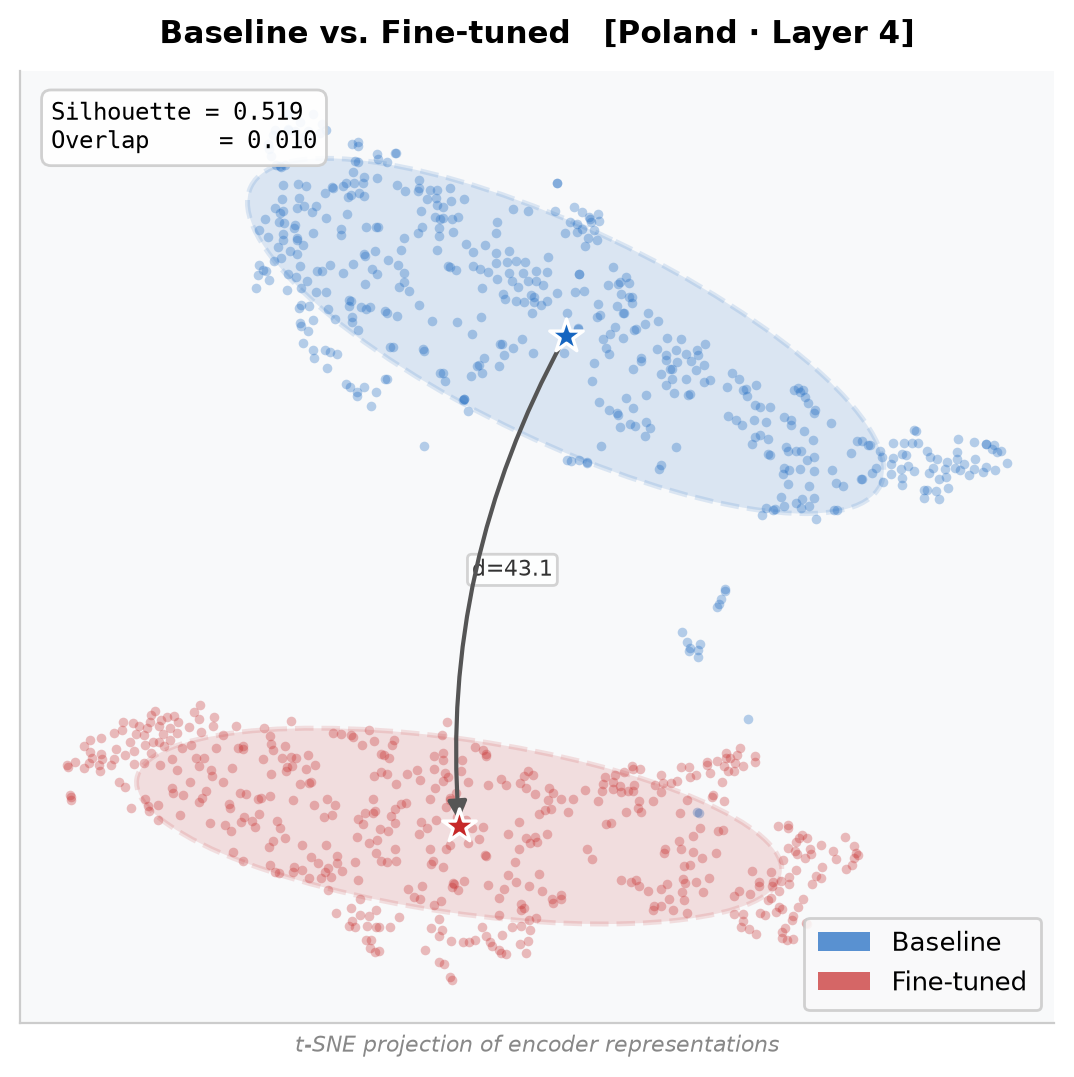
\includegraphics[width=\linewidth]{images/tsne_poland_baseline_vs_poland_transfer.png}
    \end{minipage}
    \hfill
    \begin{minipage}[t]{0.32\linewidth}
        \centering
        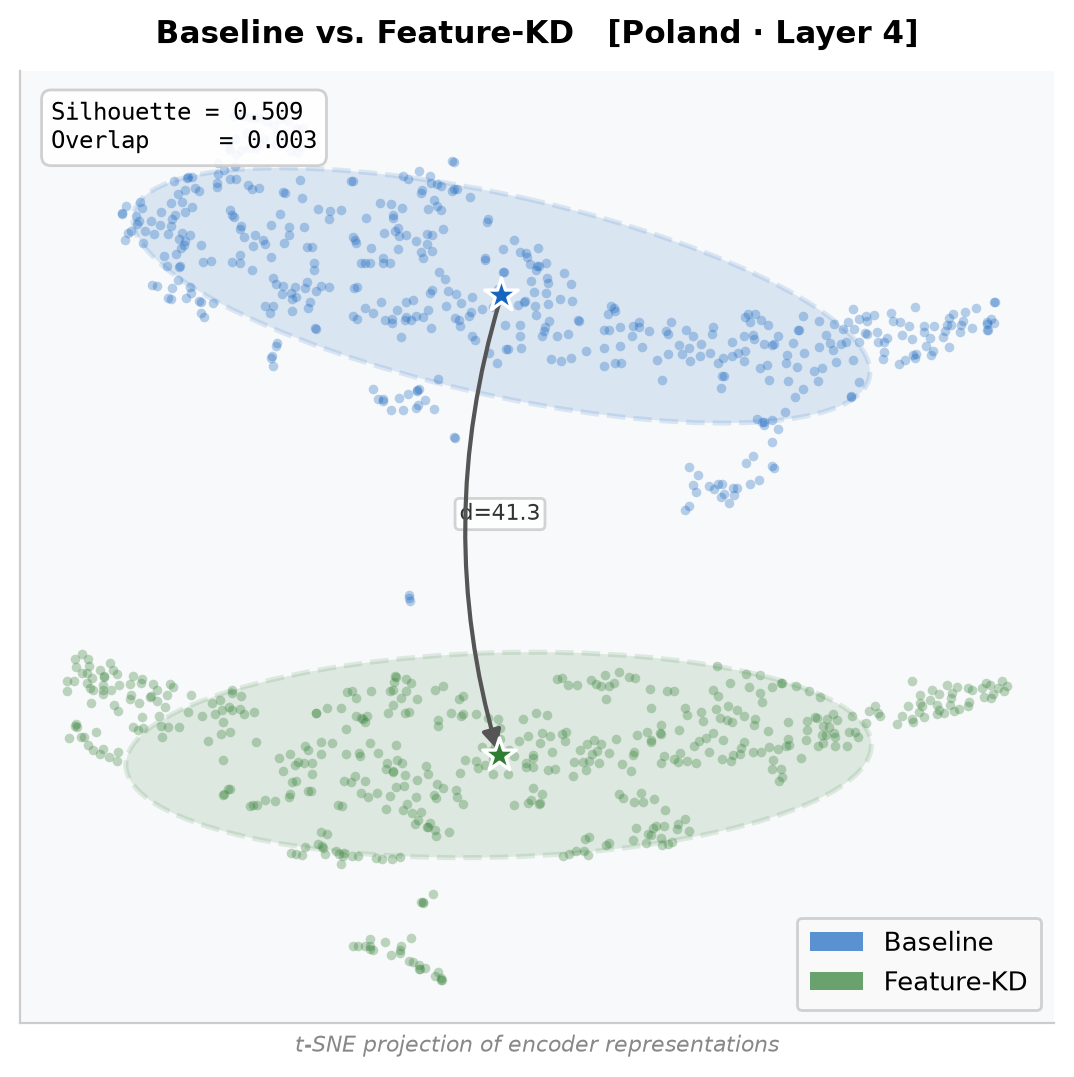
\includegraphics[width=\linewidth]{images/tsne_poland_baseline_vs_poland_feature.png}
    \end{minipage}
    \hfill
    \begin{minipage}[t]{0.32\linewidth}
        \centering
        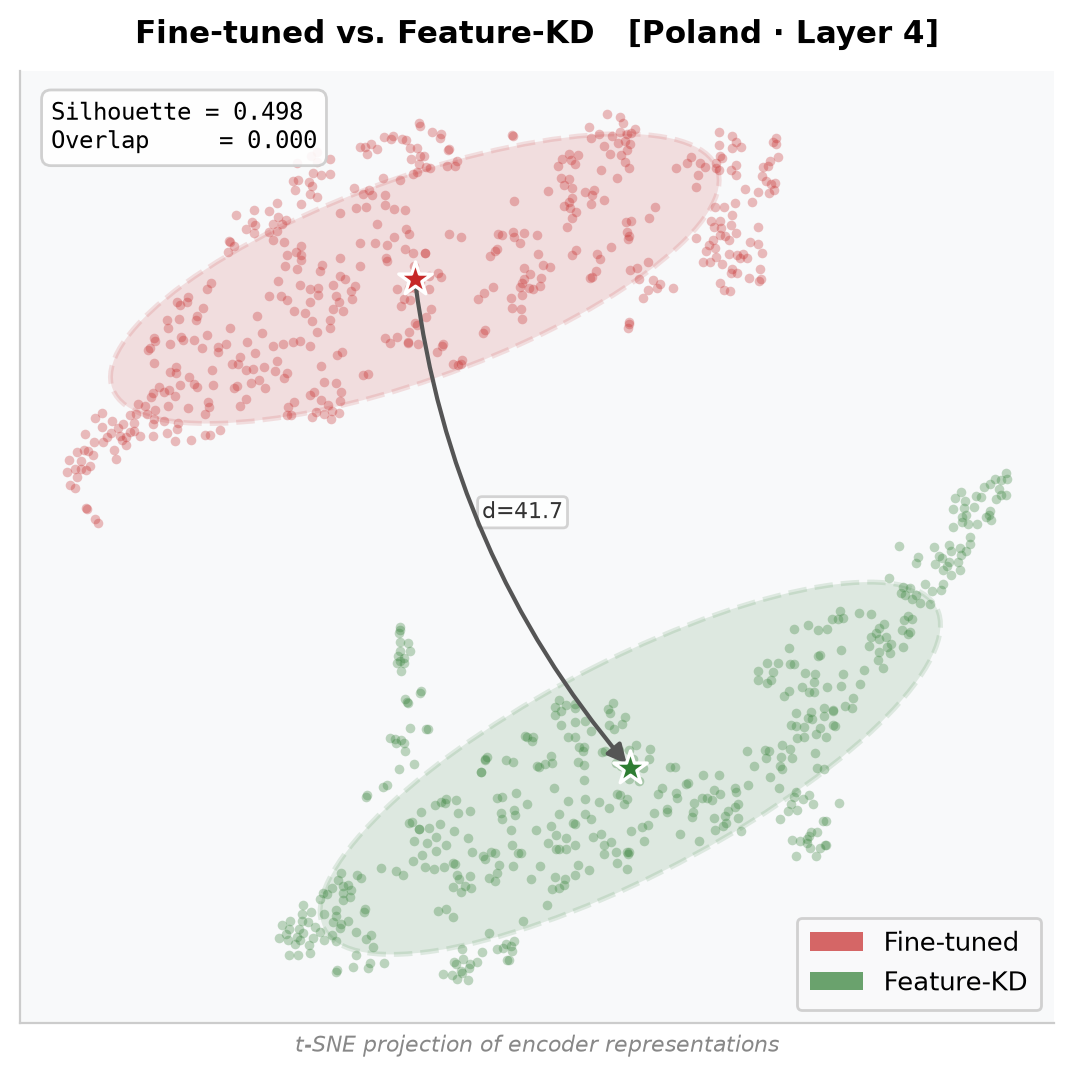
\includegraphics[width=\linewidth]{images/tsne_poland_transfer_vs_poland_feature.png}
    \end{minipage}
    % \hfill
    
    \begin{minipage}[t]{0.32\linewidth}
        \centering
        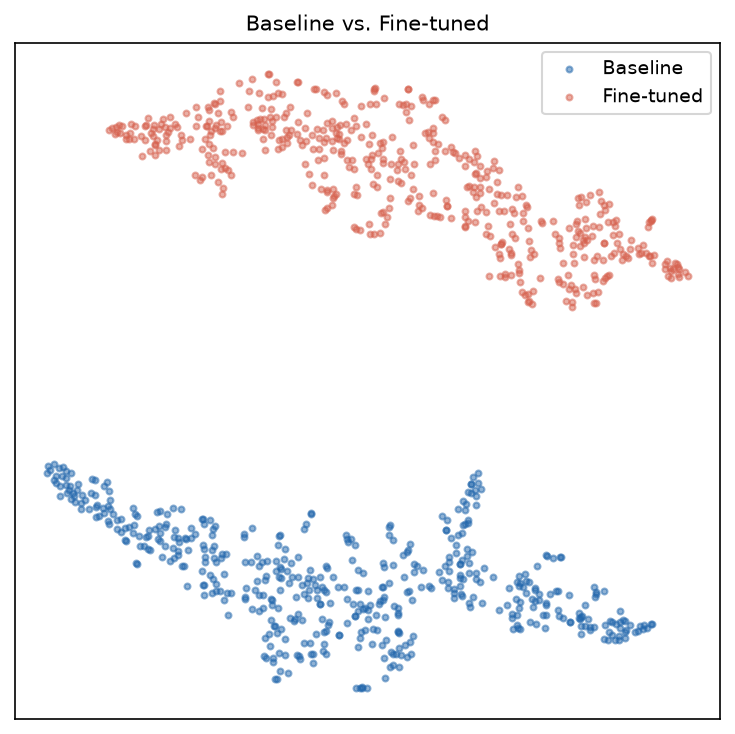
\includegraphics[width=\linewidth]{images/tsne_finland_baseline_vs_finland_transfer.png}
    \end{minipage}
    % \hfill
    \begin{minipage}[t]{0.32\linewidth}
        \centering
        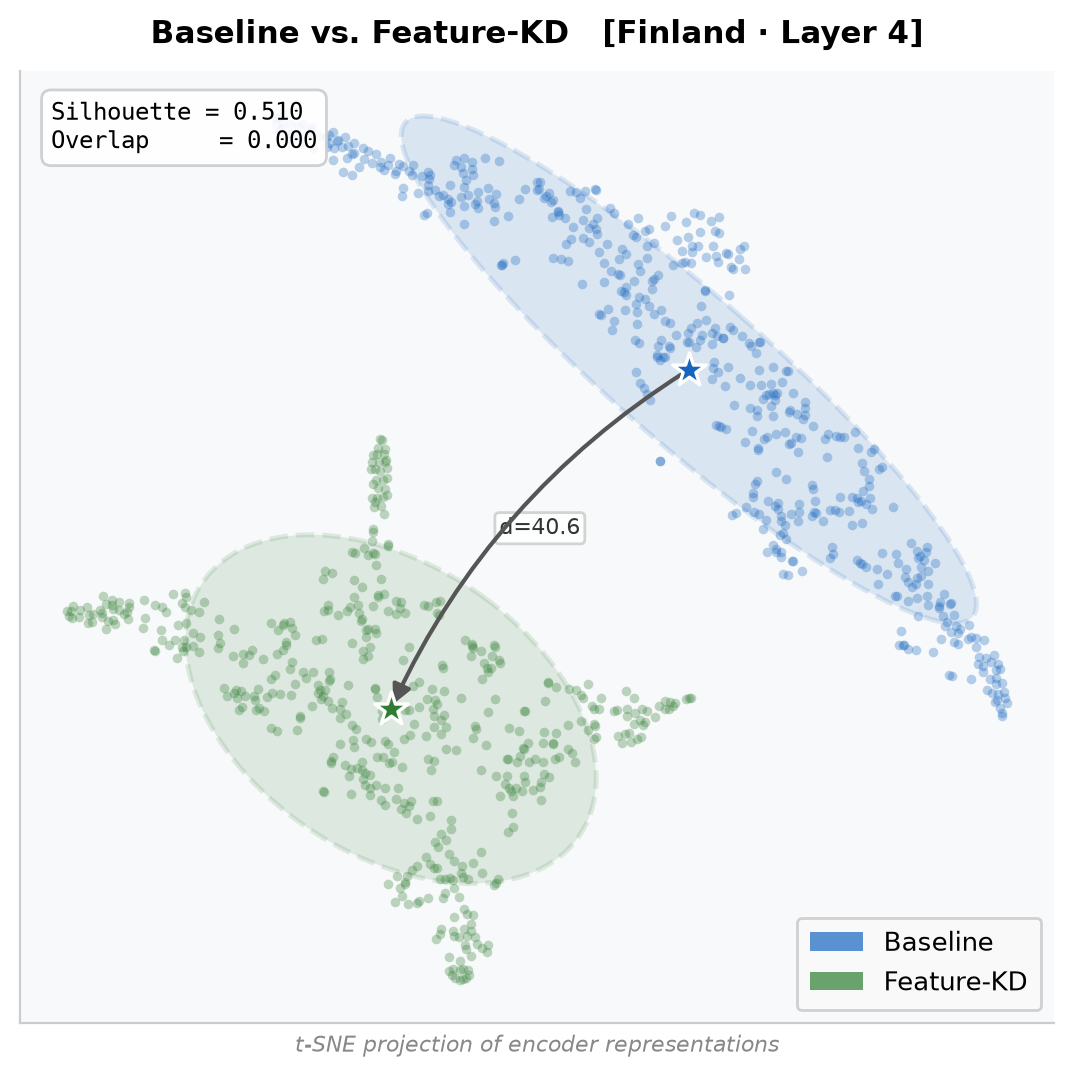
\includegraphics[width=\linewidth]{images/tsne_finland_baseline_vs_finland_feature.png}
    \end{minipage}

    \caption{t-SNE visualizations of layer4 features comparing model pairs across Poland and Finland datasets.}
    \label{fig:tsne_scatterplots}
\end{figure*}

\begin{table}[!t]
    \def\arraystretch{1.1}
    \centering
    \footnotesize
    \caption{t-SNE cluster metrics for model pairs on Polish and Finnish datasets. Model pairs are abbreviated as: B vs. F (\textit{Baseline} vs. \textit{Fine-tuned}), B vs. KD (\textit{Baseline} vs. Feature-KD), and F vs. KD (\textit{Fine-tuned} vs. Feature-KD).}
    \begin{adjustbox}{max width=0.9\columnwidth}
    \begin{tabular}{llccccc}
    \toprule
    & \textsc{\shortstack{Model\\Pair}} & 
    \textsc{\shortstack{Silhouette\\Score}} & \textsc{\shortstack{Centroid\\Distance}} & \textsc{\shortstack{Compactness\\Model A}} & \textsc{\shortstack{Compactness\\Model B}} & \textsc{\shortstack{Domain\\Overlap Ratio}} \\
    \midrule
    \multicolumn{7}{l}{\texttt{Poland}} \\
    & B vs. F  & 0.108 & 17.258 & 31.899 & 32.650 & 0.228 \\
    & B vs. KD & 0.096 & 16.019 & 30.560 & 36.884 & 0.223 \\
    & F vs. KD & 0.003 &  2.777 & 39.944 & 44.767 & 0.491 \\
    \midrule
    \multicolumn{7}{l}{\texttt{Finland}} \\
    & B vs. F  & 0.203 & 25.938 & 33.388 & 28.997 & 0.180 \\
    & B vs. KD & 0.173 & 22.403 & 32.664 & 30.170 & 0.174 \\
    \bottomrule
    \end{tabular}
    \end{adjustbox}
    \label{tbl:tsne_metrics}
\end{table}

\mypar{Linear Probing for Representation Quality}:
Linear probing results in Figure~\ref{fig:linear_probing} evaluate separability. On Finland, the \textit{Baseline} shows stable performance (acc $\sim$0.80--0.83, auc $\sim$0.86--0.93), peaking in Layer 2. On Poland, both adapted models improve with depth: \textit{Fine-tuned} reaches acc/f1 0.85 and auc 0.94 in Layer 4, while \textit{Feature-level KD} outperforms in deeper layers (Layer 4: acc 0.87, f1 0.88, auc 0.95) and Layer 1 (acc 0.81 vs. 0.78). This suggests KD yields more linearly separable representations, particularly in semantic layers, correlating with its higher cross-domain consistency.

\begin{figure}[!t]
    \centering
    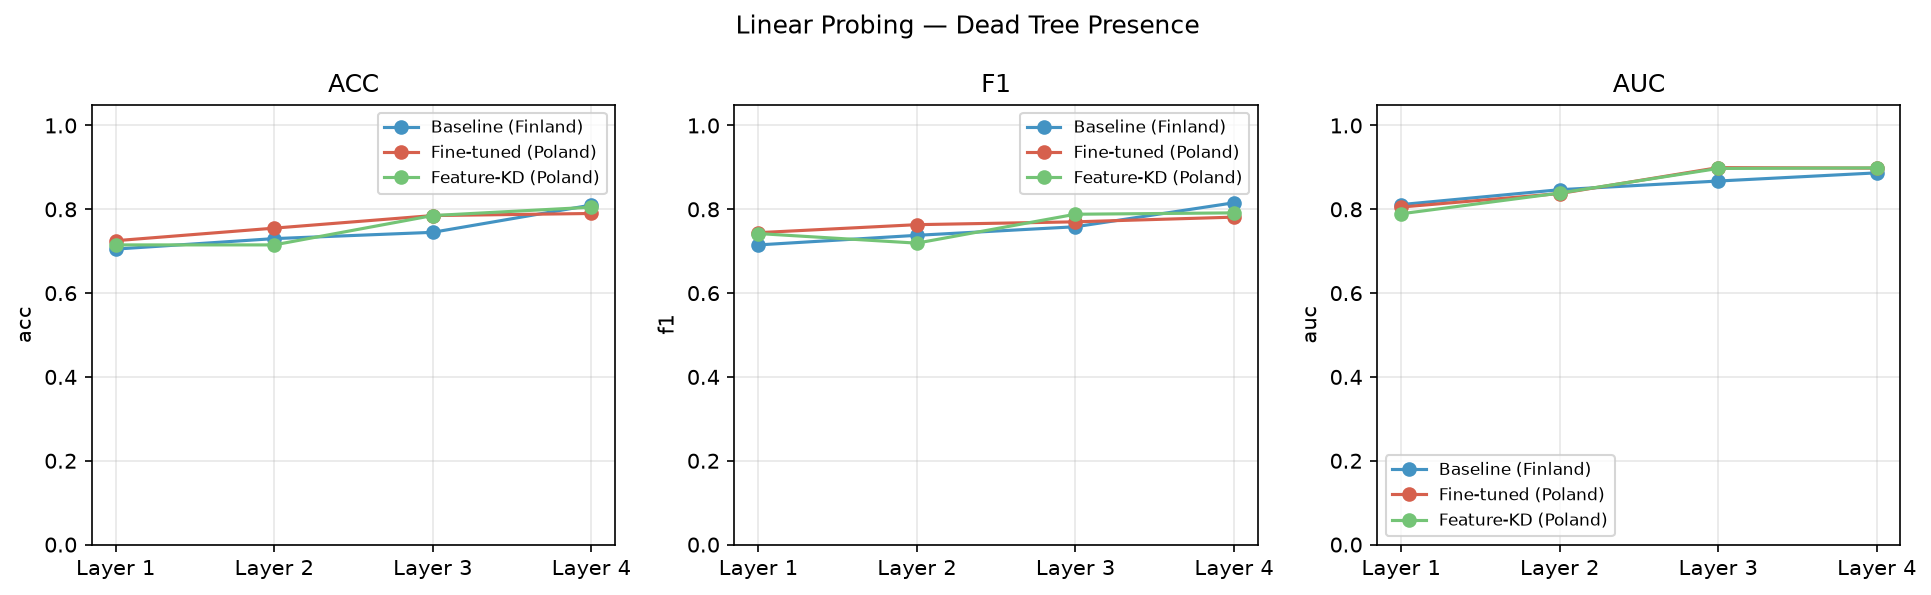
\includegraphics[width=\linewidth]{images/linear_probe.png}
    \caption{Linear probing results across layers for models on their respective datasets (\textit{Baseline} on Finland; \textit{Fine-tuned} and Feature-KD on Poland). Bold values indicate the highest per metric and layer.}
    \label{fig:linear_probing}
\end{figure}

In summary, KD variants consistently outperform fine-tuning on Tree IoU, with Self KD leading on Poland (0.277) and Germany (0.328) and Feature-level KD leading on Estonia (0.265). All KD methods outperform DANN, which itself provides only modest gains over fine-tuning. Feature-level KD exhibits superior representational invariance (higher deep-layer CKA/SSIM, better domain mixing in t-SNE, linear probing AUC 0.95), positioning it as a promising tool for precision-critical forestry monitoring.

\section{Discussion}
\label{sec:discussion}

The results highlight distinct strengths and trade-offs among fine-tuning, DANN, and KD variants for cross-domain dead tree detection. We discuss key findings and their implications for ecological monitoring.

\subsection{\textit{Fine-tuned} and DANN: Supervised Baselines}
Fine-tuning achieves a Poland Tree IoU of 0.216 with centroid F1-score 0.667, demonstrating that supervised adaptation provides substantial gains over zero-shot transfer. However, 2,105 missed trees (Tree FN) indicate that domain mismatch remains a significant limiting factor. Fine-tuning is well-suited for exhaustive surveying tasks where completeness matters more than precision, such as post-disturbance mortality assessments. DANN (Tree IoU 0.242 on Poland; centroid F1 0.702) offers a modest improvement by adversarially aligning encoder bottleneck features between Finland and the target domain. However, DANN's gains are inconsistent across countries — it fails on Germany (Tree IoU 0.083 vs.\ fine-tuning's 0.108), where resolution differences (0.10~m vs.\ 0.25~m) and the small test set (79 trees) may prevent the gradient-reversal discriminator from converging. The result confirms that adversarial feature alignment alone is insufficient when domain gaps are large and multi-scale.

\subsection{\textit{Self KD} and \textit{Basic KD}: Best Detection Accuracy}
Self KD achieves the highest Tree IoU on Poland (0.277) and Germany (0.328) by using an EMA-based self-improvement mechanism that progressively refines predictions without requiring an explicit domain alignment signal. The EMA teacher provides stable soft targets that smooth out noisy labels from annotation-sparse regions, yielding better detection of faint and partially occluded dead trees. Basic KD complements this with the lowest false positive count (1,811 Tree FP on Poland) and best centroid precision (0.713), balancing temperature-scaled soft supervision with ground-truth labels. For forestry operations requiring both high detection rates and controlled false alarms, Basic KD offers the best practical operating point.

\subsection{\textit{Feature-level KD}: Cross-Domain Precision}
Feature-level KD leads on Estonia (Tree IoU 0.265) and consistently achieves high centroid precision across all countries. Its intermediate feature alignment forces the student encoder to reproduce the teacher's latent geometry at multiple scales, yielding more domain-invariant representations as confirmed by t-SNE cluster metrics (overlap ratio 0.491) and linear probing AUC (0.95 in Layer 4). This encoder alignment is particularly valuable for the Estonian dataset, which uses CIR bands (NIR/red/green) and higher tree densities, as it transfers spectral-invariant texture features for identifying decay stages beyond what soft-label supervision alone provides. In forestry monitoring applications where false detections directly incur field-visit costs, Feature-level KD's precision advantage is operationally significant.

\subsection{Cross-Domain Robustness: KD vs.\ DANN}
Zero-shot transfer from Finland to Germany yields Tree IoU of exactly 0.000 --- the Finnish teacher detects no German trees at all, likely due to the 2.5$\times$ resolution difference (0.10~m vs.\ 0.25~m) and distinct broadleaf species composition. All KD variants recover strongly from this zero point (Self KD: 0.328), while DANN (0.083) falls even below fine-tuning (0.108), confirming that adversarial alignment cannot bridge large multi-scale domain gaps. On Poland, all KD variants exceed the zero-shot baseline (0.121) by a factor of 2.1--2.3$\times$. On Estonia, where the zero-shot teacher already performs competitively (0.219) due to similar boreal forest structure, KD further improves over zero-shot rather than degrading it --- a property that both DANN (0.205) and fine-tuning (0.202) fail to achieve. DANN's discriminator cannot provide useful gradients when the domain gap is too large or the target set too small; KD's teacher predictive distribution, by contrast, is intrinsically stable across all three conditions. These findings establish teacher-guided distillation as the most robust strategy for cross-domain dead tree detection across the boreal-to-temperate gradient.

\subsection{Data Efficiency: Performance in Low-Data Scenarios}
In low-data settings (Table~\ref{tbl:data_analysis}), Feature-level KD outperforms Fine-tuning on Tree IoU across all data fractions, with the gap persisting even at 25\% data (0.262 vs.\ 0.221). Feature-level KD at 25\% data exceeds Fine-tuning trained on the full dataset, demonstrating that teacher guidance substitutes effectively for additional annotations. This makes Feature-level KD a strong choice for remote or under-resourced forest regions where annotation budgets are limited. Linear probing reveals superior separability in KD-adapted representations even at reduced data percentages, correlating with its consistent Tree IoU advantage under annotation scarcity.

\subsection{Practical Implications for Forestry}
Field surveys of dead trees in Scandinavian and Central European forestry operations typically cost between €50--€200 per hectare, with identification precision directly determining follow-up intervention efficiency. Basic KD's reduction of false positive detections from 1,977 (fine-tuning) to 1,811 on Poland's test set — a 8.4\% decrease — translates to proportionally fewer unnecessary field visits. Feature-level KD's consistent centroid precision across Poland, Germany, and Estonia makes it particularly suitable for pan-European monitoring programs where a single model must serve heterogeneous forest types. For maximum detection coverage (e.g., post-storm or post-fire mortality mapping), Self KD is preferred given its higher Tree TP count and recall.

\subsection{Potential for On-Board Deployment}
In traditional KD, the student is more compact than the teacher, enabling edge deployment~\citep{himeur2024applications}. Here, teacher and student share the same architecture, so size reduction is not automatic. However, the distillation process significantly enhances generalization, making KD-adapted models more reliable than fine-tuned counterparts under the varied imaging conditions encountered during aerial survey flights. Future work could integrate KD with pruning or quantization to enable lightweight student models for UAV-based on-board dead tree mapping.

\subsection{Limitations and Future Directions}
This study has several limitations. First, all datasets are from European boreal and temperate forests (Finland, Poland, Germany, Estonia); performance on tropical or subtropical forests~\citep{cheng2024scattered} where dead tree appearance, canopy structure, and spectral conditions differ substantially remains untested. Second, annotations were produced by expert photointerpretation without formal inter-annotator agreement assessment; annotation uncertainty and label noise may affect both training and evaluation, particularly for trees in early decay stages whose aerial appearance closely resembles living vegetation. Third, multi-year acquisition windows (e.g., Finnish imagery spanning 2011--2023) introduce seasonal and phenological variation that may affect spectral consistency across the training set; species-specific decay rates add further ambiguity between snag (standing dead) and fresh mortality classes. Fourth, the current RGB-NIR input restricts spectral discrimination; hyperspectral or LiDAR data could reveal subtler decay signatures. Future research should address geographic scope by including diverse biomes, quantify annotation uncertainty through inter-annotator studies, and investigate hybrid KD combined with unsupervised domain adaptation for settings where labeled target data is unavailable.

\section{Conclusion}
\label{sec:conclusion}

This study presents a systematic benchmark of KD strategies for cross-domain dead tree detection, comparing four KD variants against fine-tuning and DANN domain adaptation across three European target domains. With an updated Finnish teacher (Tree IoU 0.448), all KD variants substantially outperform both baselines: Self KD achieves the highest detection accuracy on Poland (Tree IoU 0.277 vs.\ fine-tuning 0.216) and Germany (0.328 vs.\ 0.108); Feature-level KD leads on Estonia (0.265 vs.\ 0.202) and consistently reduces false positives. Crucially, all KD variants outperform DANN on every target country, demonstrating that teacher-guided soft-target transfer is more effective than adversarial feature alignment for this task. Representational analyses confirm that Feature-level KD produces more domain-invariant encoder representations (higher CKA/SSIM alignments, t-SNE domain overlap 0.491, linear probing AUC 0.95), explaining its cross-domain precision stability.

These findings establish KD — particularly Self KD for maximum accuracy and Feature-level KD for cross-domain precision — as reliable, scalable transfer strategies for ecological dead tree mapping. Future work should extend this benchmark to non-European biomes, quantify annotation uncertainty, and explore hybrid KD with compression for UAV-based on-board deployment. In summary, this work provides an actionable framework for knowledge-transfer-based forest health monitoring across diverse European forest ecosystems.

\section*{Acknowledgments}

This work was funded by the European Union (ERC-2023-STG grant agreement no. 101116404). Views and opinions expressed are, however, those of the author(s) only and do not necessarily reflect those of the European Union or the European Research Council Executive Agency. Neither the European Union nor the granting authority can be held responsible for them. The authors greatly acknowledge CSC -- IT Center for Science, Finland, for computational resources.

% --- Bibliography Section ---
% Note: arXiv requires you to submit the compiled .bbl file along with your .tex file.
\bibliographystyle{unsrtnat}
\bibliography{references} 

\end{document}